\documentclass[11pt]{article}
%\usepackage{newpxtext,newpxmath}
\usepackage[left=1in,right=1in,top=1in,bottom=1in]{geometry}
\usepackage{graphicx, amsmath, amsthm, latexsym, amssymb, color,cite,enumerate, physics, framed}
\usepackage{caption,subcaption, empheq, hyperref, xcolor}
\usepackage{mathtools}
\usepackage[titletoc]{appendix}


\pagenumbering{arabic}
\newtheorem{theorem}{Theorem}[section]
\newtheorem{lemma}[theorem]{Lemma}
\newtheorem{definition}[theorem]{Definition}
\newtheorem{corollary}[theorem]{Corollary}
\newtheorem{proposition}[theorem]{Proposition}
\newtheorem{convention}[theorem]{Convention}
\newtheorem{conjecture}[theorem]{Conjecture}
\newtheorem{remark}{Remark}
\newtheorem{example}{Example}
\newtheorem*{solution}{Solution}
\newcommand*{\myproofname}{Proof}
\newenvironment{subproof}[1][\myproofname]{\begin{proof}[#1]\renewcommand*{\qedsymbol}{$\mathbin{/\mkern-6mu/}$}}{\end{proof}}

\newcommand{\p}{\partial}
\newcommand{\R}{\mathbb{R}}
\newcommand{\C}{\mathbb{C}}
\newcommand{\lag}{\mathcal{L}}
\newcommand{\nn}{\nonumber}
\newcommand{\ham}{\mathcal{H}}
\newcommand{\M}{\mathcal{M}}
\newcommand{\I}{\mathcal{I}}
\newcommand{\K}{\mathcal{K}}
\newcommand{\F}{\mathcal{F}}
\newcommand{\w}{\omega}
\newcommand{\lam}{\lambda}
\newcommand{\al}{\alpha}
\newcommand{\be}{\beta}
\newcommand{\x}{\xi}
\newcommand{\G}{\mathcal{G}}
\newcommand{\f}[2]{\frac{#1}{#2}}
\newcommand{\ift}{\infty}
\newcommand{\lp}{\left(}
\newcommand{\rp}{\right)}
\newcommand{\lb}{\left[}
\newcommand{\rb}{\right]}
\newcommand{\lc}{\left\{}
\newcommand{\rc}{\right\}}
\newcommand{\V}{\mathbf{V}}
\newcommand{\U}{\mathcal{U}}
\newcommand{\Id}{\mathcal{I}}
\newcommand{\D}{\mathcal{D}}
\newcommand{\Z}{\mathcal{Z}}

\hypersetup{
	colorlinks,
	linkcolor={black!50!black},
	citecolor={blue!50!black},
	urlcolor={blue!80!black}
}

% 3j symbol
\newcommand{\tj}[6]{ \begin{pmatrix}
		#1 & #2 & #3 \\
		#4 & #5 & #6 
\end{pmatrix}}
% 6j symbol
\newcommand{\Gj}[6]{ \begin{Bmatrix}
		#1 & #2 & #3 \\
		#4 & #5 & #6 
\end{Bmatrix}}



\begin{document}
\begin{center}
\textbf{HYPERFINE QUANTUM BEATS \& THE MAGIC ANGLE}\\

Huan Q. Bui\\
\today
\end{center}



\tableofcontents


\newpage


\section{Introduction}
This document details some theory related to quantum beats, which occur in and can affect radiative lifetime measurements. Most of the mathematical ideas are synthesized from ``\textit{Hyperfine-structure quantum beats: application of the graphical methods of angular-momentum theory to the calculation of intensity profiles}'' by Luypaert and Van Craen (1977) and Section 7.2: Quantum Beat Theory in the Density Matrix Formalism in ``\textit{Quantum Beats and Time-Resolved Fluorescence Spectroscopy}'' by S. Haroche (1976).


\begin{figure}[!htb]
	\centering
	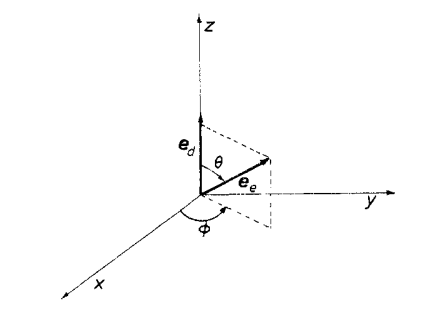
\includegraphics[scale=0.7]{beats_1}
	\caption{ Excitation-detection geometry using linear polarizers \cite{Luypaert_1977}.}
	\label{fig:scheme}
\end{figure}




\section{The Magic-Angle Problem}
Problem 9.4 of \cite{demille_atoms} on polarized fluorescence: Consider an experiment where atoms are excited with linearly polarized light, and the emitted light passes through a linear polarizer before reaching the detector. Show that if the polarization vector of the exciting light forms the ``magic angle'' $\theta_m$ given by:
\begin{equation*}
\theta_m = \arccos(1/\sqrt{3}) \approx 54.74^\circ
\end{equation*}
with the axis of the linear polarizer in front of the detector, then the detected signal is insensitive to the anisotropic part of the fluorescence. 


\begin{solution}
	\normalfont{Here's the \textit{qualitative} solution, taken from \cite{demille_atoms}. A more complete treatment of this problem is outlined in the following sections and appendices. 
	

	To start, we assume weak and broadline/broadband excitation. Assume further that the ground state is initially unpolarized. Since the excitation light is linearly polarized, the excited state is that of a photon (this will be justified in better detail). This implies that the density matrix of the excited state has no \textit{orientation} ($k=1$) component. This leaves us with the \textit{population} $(k=0)$ and \textit{alignment} $(k=2)$ terms. As we will see, only the alignment term contributes to radiation anisotropy. This anisotropy corresponds to $k=2, q=0$, where $k,q$ correspond to the tensor rank and component, respectively. The Wigner-Eckart theorem leads us to the following expression for the radiation intensity:
	\begin{equation*}
	I(t)\propto A  +B(t)P_2(\cos\theta)
	\end{equation*} 
	where $\theta$ is the angle between the radiated and detected polarization. Here, $A$ and $B(t)$ depends on the system and are not necessarily non-zero. This states that the radiation has no $\phi$-dependence, and that quantum beats arise when $P_2(\cos\theta) \neq 0$. When $\theta = \theta_m$, this part vanishes. 
	
	Discussions of tensor expansions and the details related to this problem can be found below and in \cite{haroche}, \cite{Luypaert_1977}, \cite{angular_momentum}.
	}
\end{solution}






\section{Some quantum-beat theory}\label{sec:beat_theory}

Roughly speaking, quantum beats occur due to ``interference'' in the decay of a coherent superposition of closely-spaced atomic states $\{\ket{{e}}\}$ to some collection of the final states $\{ \ket{{f}}  \}$, where $\{ \ket{{e}}   \}$ is obtained by an pulsed laser with pulse duration $\Theta \ll \tau$, the mean lifetime of $\{ \ket{{e}}   \}$. The basic scheme is given by Figure \ref{fig:energies}.

\begin{figure}[!htb]
	\centering
	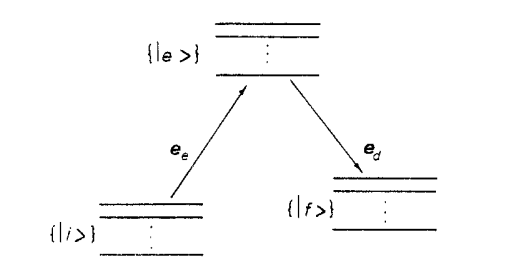
\includegraphics[scale=0.7]{energies}
	\caption{Typical quantum-beat scheme \cite{Luypaert_1977}.}
	\label{fig:energies}
\end{figure}


A short pulse of resonant light of polarization $\mathbf{e}_e$ excites an ensemble of atoms from a set of initial states $\{ \ket{i}  \}$ to $\{ \ket{e} \}$. The decay $\{ \ket{e} \} \to\{ \ket{f}  \}$ generates fluorescence light with intensity $I_{\tiny{\mbox{tot}}}(t)$. We are interested in the intensity $I(t)$ of a particular polarization $\mathbf{e}_d$ of $I_{\tiny{\mbox{tot}}}(t)$.  


In general (see Appendix \ref{app:quantum_beats}), we have
\begin{equation}\label{eq:intensity}
I(t) \propto \Tr_e\{   \rho_e(t) \mathfrak{D}  \},
\end{equation}
where $\rho_e(t)$ is the density matrix of the excited state describing the time evolution of the excited state after the pulse, and $\mathfrak{D}$ is the detection operator given in terms of the scaled-electric-dipole operator $\mathbf{D}$ as 
\begin{equation}\label{eq:detection}
\mathfrak{D} = \sum_f (\mathbf{e}_d \cdot \mathbf{D}) \ket{f}\bra{f}(\mathbf{e}_d^* \cdot \mathbf{D}).
\end{equation}
$\rho_e(t)$ is simple so long as the following conditions are satisfied:
\begin{itemize}
	\item The excitation is broadline, i.e., the spectral width of the exciting light is much bigger than the inverse of the duration of the pulse. 
	\item The excitation is weakly-coupled to the atomic system, i.e., the duration of the pulse is much less than the average time between two successive photon absorptions by an atom. 
	\item The duration of the pulse is shorter than the mean lifetime $\tau$ of $\{ \ket{e} \}$, and is less than the inverse Bohr frequencies $\omega_{e,e'}$ corresponding to the excited-state energy differences. 
\end{itemize}
Under these conditions \textcolor{blue}{(which I believe our experiment satisfies)}, the density matrix $\rho_e(t)$ has the following property:
\begin{equation}\label{eq:density}
\bra{e} \rho_e(t) \ket{e'} = \sum_{ii'} \bra{e} \mathbf{e}_e \cdot \mathbf{D} \ket{i} \bra{i} \rho_i(-T) \ket{i'} \bra{i'} \mathbf{e}_e^* \cdot \mathbf{D} \ket{e'} \exp\lb -(i\omega_{ee'} + \Gamma_e) t \rb,
\end{equation}
where $\rho_i(-T)$ is the density matrix of the initial state. Here, $\Gamma_e = \tau_e^{-1}$. Putting Eq. \ref{eq:density} into Eq. \ref{eq:intensity} and Eq. \ref{eq:detection} we find
\begin{align}\label{eq:Intensity_full}
I(t) \propto \sum_{f,ii',ee'} &\bra{e} \mathbf{e}_e \cdot \mathbf{D} \ket{i} \bra{i} \rho_i(-T) \ket{i'} \bra{i'} \mathbf{e}_e^* \cdot \mathbf{D} \ket{e'} \nonumber \\
&\times \bra{e'}\mathbf{e}_d \cdot \mathbf{D} \ket{f}\bra{f}\mathbf{e}_d^* \cdot \mathbf{D} \ket{e} \exp\lb -(i\omega_{ee'} + \Gamma_e) t \rb.
\end{align}
This corresponds exactly to Eq. \ref{eq:signal_full} in Appendix \ref{app:quantum_beats}. For a detailed derivation of this equation, see the rest of Appendix \ref{app:quantum_beats}, where the symbol for initial states $i$ becomes $g$. 





\section{Hyperfine-structure quantum beats}
Now we focus on quantum beats due to hyperfine splitting. The atoms are assumed to have a non-zero nuclear spin. \textcolor{blue}{In our case, $I_K = 3/2$.} In this case, the atomic states will be represented by 
\begin{equation}
\ket{a} = \ket{\al(J_a I) F_a M_a} \equiv \ket{F_a M_a}, \quad a = i,e,f.
\end{equation}
$J_a$ denotes the total electronic angular momentum, $I$ the nuclear spin, $F_a$ the total angular momentum and $M_a$ the quantum number corresponding to its projection on the $z$-axis. Finally, $\al$ stands for all other labels necessary to identify each state. We assume that initially, the ground state is unpolarized (or \textit{totally mixed}), i.e., that $\rho_i(-T) \propto \mathbb{I}$, the identity matrix. In this case, the intensity $I(t)$ is slightly simplified:
\begin{align}
I(t) \propto &\sum_{F_eM_e,F'_eM'_e,F_iM_i,F_fM_f} \bra{F_eM_e} \mathbf{e}_e \cdot \mathbf{D} \ket{F_iM_i} \bra{F_iM_i}  \bra{F_i M_i} \mathbf{e}_e^* \cdot \mathbf{D} \ket{F'_eM'_e} \nonumber \\
&\times \bra{F'_eM'_e}\mathbf{e}_d \cdot \mathbf{D} \ket{F_fM_f}\bra{F_fM_f}\mathbf{e}_d^* \cdot \mathbf{D} \ket{F_eM_e} \exp\lb -(i\omega_{F_eF'_e} + \Gamma_e) t \rb.
\end{align}
The next step is to eliminate irrelevant quantum numbers in order to make the dependence on the characteristics of the atom more explicit. To this end, we will eliminate the quantum numbers $M_F$ and sum over all $F_i, F_f$. Eliminating $M_F$'s requires reducing the electric-dipole matrix elements. We do this by making use of the Wigner-Eckart theorem and known reduction formulas. First, we eliminate the dependence on the $M_F$ quantum numbers:
\begin{align*}
\bra{F_e M_e} \mathbf{e}_e \cdot \mathbf{D} \ket{F_i M_i}
&=  \sum_{p_0} (\mathbf{e}_e)_{p_0} \bra{F_e M_e} \mathbf{D}_{p_0} \ket{F_i M_i}\\
&= \sum_{p_0} (\mathbf{e}_e)_{p_0} (-1)^{F_e - M_e} \tj{F_e}{1}{F_i}{-M_e}{p_0}{M_i} \bra{F_e} \abs{\mathbf{D}} \ket{F_i}\\
&= \sum_{p_0} (\mathbf{e}_e)_{p_0} (-1)^{F_e - M_e} \tj{F_e}{1}{F_i}{-M_e}{p_0}{M_i} \bra{(J_e I) F_e} \abs{\mathbf{D}} \ket{(J_i I)F_i}.
\end{align*}
Similarly, we find 
\begin{align*}
\bra{F_i M_i} \mathbf{e}^*_e \cdot \mathbf{D} \ket{F'_e M'_e}
&=  \sum_{p'_0} (\mathbf{e}_e^*)_{p'_0} \bra{F_i M_i} \mathbf{D}_{p'_0} \ket{F'_e M'_e}\\
&= \sum_{p'_0} (\mathbf{e}^*_e)_{p'_0} (-1)^{F_i - M_i} \tj{F_i}{1}{F'_e}{-M_i}{p'_0}{M'_e} \bra{F_i} \abs{\mathbf{D}} \ket{F'_e}\\
&= \sum_{p'_0} (\mathbf{e}^*_e)_{p'_0} (-1)^{F_i - M_i} \tj{F_i}{1}{F'_e}{-M_i}{p'_0}{M'_e} \bra{(J_i I)F_i} \abs{\mathbf{D}} \ket{(J_e I)F'_e}.
\end{align*}
\begin{align*}
\bra{F'_e M'_e} \mathbf{e}_d \cdot \mathbf{D} \ket{F_f M_f}
&=  \sum_{p} (\mathbf{e}_d)_{p} \bra{F'_e M'_e} \mathbf{D}_{p} \ket{F_f M_f}\\
&= \sum_{p} (\mathbf{e}_d)_{p} (-1)^{F'_e - M'_e} \tj{F'_e}{1}{F_f}{-M'_e}{p}{M_f} \bra{F_e'} \abs{\mathbf{D}} \ket{F_f}\\
&= \sum_{p} (\mathbf{e}_d)_{p'_0} (-1)^{F'_e - M'_e} \tj{F'_e}{1}{F_f}{-M'_e}{p}{M_f} \bra{(J_e I)F_e'}\abs{\mathbf{D}} \ket{(J_f I)F_f}
\end{align*}
\begin{align*}
\bra{F_f M_f} \mathbf{e}^*_d \cdot \mathbf{D} \ket{F_e M_e}
&=  \sum_{p'} (\mathbf{e}_d^*)_{p'} \bra{F_f M_f} \mathbf{D}_{p'} \ket{F_e M_e}\\
&= \sum_{p'} (\mathbf{e}^*_d)_{p'} (-1)^{F_f - M_f} \tj{F_f}{1}{F_e}{-M_f}{p'}{M_e} \bra{F_f} \abs{\mathbf{D}} \ket{F_e}\\
&= \sum_{p'} (\mathbf{e}^*_d)_{p'} (-1)^{F_f - M_f} \tj{F_f}{1}{F_e}{-M_f}{p'}{M_e} \bra{(J_f I)F_f} \abs{\mathbf{D}} \ket{(J_e I)F_e}.
\end{align*}
Next, we further reduce the matrix elements $\bra{(J'I)F'} \mathcal{O} \ket{(J I) F}$, introducing the $6j$-symbol:
\begin{align*}
\bra{(J_e I) F_e} \abs{\mathbf{D}} \ket{(J_i I)F_i}
&= (-1)^{J_e + I + F_i + 1}\sqrt{(2F_e + 1)(2F_i+1)} 
\Gj{J_e}{F_e}{I}{F_i}{J_i}{1}\bra{J_e}\abs{\mathbf{D}} \ket{J_i} \\
&= (-1)^{J_e + I + F_i + 1}\sqrt{(2F_e + 1)(2F_i+1)} 
\Gj{F_e}{F_i}{1}{J_i}{J_e}{I}\bra{J_e}\abs{\mathbf{D}} \ket{J_i},
\end{align*}
where we have used symmetry relations of the $6j$-symbol on the last line. Similarly, we find that
\begin{align*}
\bra{(J_i I)F_i} \abs{\mathbf{D}} \ket{(J_e I)F'_e}
= (-1)^{J_i + I + F_e' + 1}\sqrt{(2F_i + 1)(2F_e'+1)} 
\Gj{F_i}{F'_e}{1}{J_e}{J_i}{I}\bra{J_i}\abs{\mathbf{D}} \ket{J_e}.
\end{align*}
\begin{align*}
\bra{(J_e I)F_e'}\abs{\mathbf{D}} \ket{(J_f I)F_f}
= (-1)^{J_e + I + F_f + 1}\sqrt{(2F'_e + 1)(2F_f+1)} 
\Gj{F'_e}{F_f}{1}{J_f}{J_e}{I}\bra{J_e}\abs{\mathbf{D}} \ket{J_f}.
\end{align*}
\begin{align*}
\bra{(J_f I)F_f} \abs{\mathbf{D}} \ket{(J_e I)F_e}
= (-1)^{J_f + I + F_e + 1}\sqrt{(2F_f + 1)(2F_e+1)} 
\Gj{F_f}{F_e}{1}{J_e}{J_f}{I}\bra{J_f}\abs{\mathbf{D}} \ket{J_e}.
\end{align*}
Putting these together, we can write the signal $I(t)$ as
\begin{align}\label{eq:I(t)}
I(t) 
\propto 
\sum_{\substack{F_e, F'_e\\pp', p_0p'_0\\F_i, F_f}}
&(-1)^{p_0 + p'_0 + p + p' + F_e + F_e' + F_i + F_f}
(2F_e + 1)(2F'_e+1)(2F_i + 1)(2F_f+1)\\
& \times (\mathbf{e}_e)_{p_0}(\mathbf{e}^*_e)_{p_0'}(\mathbf{e}_d)_{p}(\mathbf{e}_d^*)_{p'} \exp\lb -(i\omega_{F_eF'_e} + \Gamma_e)t \rb\abs{\bra{J_e} \abs{\mathbf{D}}\ket{J_i}}^2\abs{ \bra{J_e} \abs{\mathbf{D}} \ket{J_f}}^2\\
&\times \Gj{F_e}{F_i}{1}{J_i}{J_e}{I}\Gj{F_i}{F'_e}{1}{J_e}{J_i}{I}\Gj{F'_e}{F_f}{1}{J_f}{J_e}{I}\Gj{F_f}{F_e}{1}{J_e}{J_f}{I}\\
&\times \sum_{\substack{M_eM'_e\\ M_i M_f}}(-1)^{F_e - M_e + F'_e - M'_e + F_i - M_i + F_f - M_f} \tj{F_e}{1}{F_i}{-M_e}{p_0}{M_i}\tj{F_i}{1}{F'_e}{-M_i}{p'_0}{M'_e}\\
&\times \tj{F'_e}{1}{F_f}{-M'_e}{p}{M_f}\tj{F_f}{1}{F_e}{-M_f}{p'}{M_e}.
\end{align}
Let 
\begin{align*}
X(F_e,F'_e,F_i,F_f;p_0.p_o',p,p') &= \sum_{\substack{M_eM'_e\\ M_i M_f}}(-1)^{F_e - M_e + F'_e - M'_e + F_i - M_i + F_f - M_f} \tj{F_e}{1}{F_i}{-M_e}{p_0}{M_i}\\ 
&\quad \times 
\tj{F_i}{1}{F'_e}{-M_i}{p'_0}{M'_e}
\tj{F'_e}{1}{F_f}{-M'_e}{p}{M_f}
\tj{F_f}{1}{F_e}{-M_f}{p'}{M_e}.
\end{align*}
We will simplify this expression, using graphical methods for angular-momentum theory from \cite{angular_momentum}. Some of the rules used in the following calculation are summarized in Appendix \ref{app:angular_momentum}. From Appendix \ref{app:X}, we find 
\begin{align*}
X(F_e,F'_e,F_i,F_f;p_0.p_o',p,p') 
&= \sum_{kq} (2k+1) 
(-1)^{q + 2F_f - F_e -F_e'}
\tj{1}{1}{k}{p_0}{p_0'}{q}\tj{1}{1}{k}{p}{p'}{-q}  \\
&\quad\times \Gj{F_i}{F_e}{1}{k}{1}{F_e'} \Gj{1}{k}{1}{F_e}{F_f}{F_e'},
\end{align*}
where $q$ are the $z$-projected quantum numbers of $k$. Plugging this expression into Eq. \ref{eq:I(t)} we find 
\begin{align*}
I(t) 
&\propto
\sum_{\substack{F_e, F'_e\\pp', p_0p'_0\\kq}}
\sum_{F_i, F_f}
(-1)^{q + 2F_f + p_0 + p'_0 + p + p'  + F_i + F_f}
(2k+1)(2F_e + 1)(2F'_e+1)\\
&\times (2F_i + 1)(2F_f+1)
(\mathbf{e}_e)_{p_0}(\mathbf{e}^*_e)_{p_0'}(\mathbf{e}_d)_{p}(\mathbf{e}_d^*)_{p'} \exp\lb -(i\omega_{F_eF'_e} + \Gamma_e)t \rb\abs{\bra{J_e} \abs{\mathbf{D}}\ket{J_i}}^2\abs{ \bra{J_e} \abs{\mathbf{D}} \ket{J_f}}^2\\
&\times \Gj{F_e}{F_i}{1}{J_i}{J_e}{I}\Gj{F_i}{F'_e}{1}{J_e}{J_i}{I}\Gj{F'_e}{F_f}{1}{J_f}{J_e}{I}\Gj{F_f}{F_e}{1}{J_e}{J_f}{I}\Gj{F_i}{F_e}{1}{k}{1}{F_e'} \Gj{1}{k}{1}{F_e}{F_f}{F_e'}\\
&\times \tj{1}{1}{k}{p_0}{p_0'}{q}\tj{1}{1}{k}{p}{p'}{-q}.
\end{align*}
We can simplify this. Notice that the selection rules on the $3j$-symbols require that $p_0 + p_0' + q = 0 = p + p' - q$. This means that
\begin{equation*}
p_0 + p_0' + p + p' = 0.
\end{equation*}
Moreover, let 
\begin{equation*}
Y(F_e, F_e';k) = \sum_{F_i}(2F_i + 1)(-1)^{2J_e + k + F_e + F_e' + I + J_i + F_i}
\Gj{F_e}{F_i}{1}{J_i}{J_e}{I}
\Gj{F_e'}{F_i}{1}{1}{k}{F_e}
\Gj{I}{F_i}{J_i}{1}{J_e}{F_e'}.
\end{equation*}
and
\begin{equation*}
Z(F_e, F_e';k) = \sum_{F_f}(2F_f + 1)(-1)^{2J_e + k + F_e + F_e' + I + J_f + F_f}
\Gj{F'_e}{F_f}{1}{J_f}{J_e}{I}
\Gj{F_e}{F_f}{1}{1}{k}{F_e'}
\Gj{I}{F_f}{J_f}{1}{J_e}{F_e}.
\end{equation*}
To write $I(t)$ in terms of $Y,Z$, we must perform some permutations within the $6j$-symbols. This brings out some phase factors \textcolor{blue}{(I will skip the details here)}. After multiple simplifications we find
\begin{align} \label{eq:bigI}
I(t) 
&\propto
\sum_{\substack{F_e, F'_e\\pp', p_0p'_0\\kq}}
(-1)^{q - J_i + J_f}
(2k+1)
\abs{\bra{J_e} \abs{\mathbf{D}}\ket{J_i}}^2\abs{ \bra{J_e} \abs{\mathbf{D}} \ket{J_f}}^2 
\exp\lb -(i\omega_{F_eF'_e} + \Gamma_e)t \rb 
(2F_e+1)\nonumber\\
&\times 
(2F'_e+1)
(\mathbf{e}_e)_{p_0}(\mathbf{e}^*_e)_{p_0'}(\mathbf{e}_d)_{p}(\mathbf{e}_d^*)_{p'} 
\tj{1}{1}{k}{p_0}{p_0'}{q}
\tj{1}{1}{k}{p}{p'}{-q}
Y(F_e,F_e';k)Z(F_e,F_e';k).
\end{align}
The next step is to calculate $Y(F_e,F_e';k)$ and $Z(F_e, F_e';k)$, again using graphical methods (see Appendix \ref{app:YZ}). Once that is done, we find 
\begin{align*}
Y(F_e, F_e';k) 
=
\Gj{k}{J_e}{J_e}{I}{F_e}{F_e'} 
\Gj{k}{J_e}{J_e}{J_i}{1}{1}
=
\Gj{F_e}{F_e'}{k}{J_e}{J_e}{I} 
\Gj{1}{1}{k}{J_e}{J_e}{J_i}
\end{align*}
and
\begin{align*}
Z(F_e, F_e';k) 
=
\Gj{k}{J_e}{J_e}{I}{F_e}{F_e'} 
\Gj{k}{J_e}{J_e}{J_f}{1}{1}
=
\Gj{F_e'}{F_e}{k}{J_e}{J_e}{I} 
\Gj{1}{1}{k}{J_e}{J_e}{J_f}.
\end{align*}
Plugging these results back into Eq. \ref{eq:bigI} we get
\begin{align}\label{eq:full_I}
I(t) \propto (-1)^{J_i - J_f}&\abs{\bra{J_e} \abs{\mathbf{D}}\ket{J_i}}^2\abs{ \bra{J_e} \abs{\mathbf{D}} \ket{J_f}}^2 \nonumber\\
&\times \sum_{\substack{kq\\F_eF_e'}} 
(-1)^q E^k_q U^k_{-q}A^k(F_eF_e')B^k(F_e'F_e)\exp\lb -(i\omega_{F_eF'_e} + \Gamma_e)t \rb 
\end{align}
where
\begin{align*}
&E^k_q 
= \sqrt{2k+1} \sum_{p_0p_0'} \tj{1}{1}{k}{p_0}{p_0'}{q}
(\mathbf{e}_e)_{p_0}(\mathbf{e}^*_e)_{p_0'}\\
&U^k_{-q} 
= \sqrt{2k+1} \sum_{pp'} \tj{1}{1}{k}{p}{p'}{-q}
(\mathbf{e}_d)_{p}(\mathbf{e}_d^*)_{p'} \\
&A^k(F_eF_e') = \sqrt{(2F_e+1)(2F_e'+1)}
\Gj{F_e}{F_e'}{k}{J_e}{J_e}{I} 
\Gj{1}{1}{k}{J_e}{J_e}{J_i}\\
&B^k(F_e'F_e) = \sqrt{(2F_e+1)(2F_e'+1)}
\Gj{F_e'}{F_e}{k}{J_e}{J_e}{I} 
\Gj{1}{1}{k}{J_e}{J_e}{J_f}.
\end{align*}
Eq. \ref{eq:full_I} has all irrelevant quantum number eliminated. All of the excitation and detection polarization characteristics are contained in the terms $E^k_q$ and $U^k_{-q}$. The terms $A^k(F_eF_e')$ and $B^k(F_e'F_e)$ depend on the atomic quantum numbers and are transition-specific. The exponential term represents quantum beats. We will see that not all transition $J_i - J_e - J_f$ will exhibit quantum beats because $A^k(F_eF_e')$ and/or $B^k(F_e'F_e)$ might vanish.


\section{Example: Linearly-polarized excitation and detection}

Now we are ready to consider the excitation/detection angle dependence in the experimental geometry given in Figure \ref{fig:scheme1}.
\begin{figure}[!htb]
	\centering
	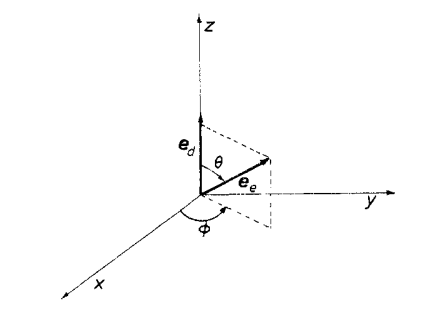
\includegraphics[scale=0.7]{beats_1}
	\caption{ Excitation-detection geometry using linear polarizers \cite{Luypaert_1977}.}
	\label{fig:scheme1}
\end{figure}
Let the $z$-axis be defined by the polarization of the detection pulse $\mathbf{e}_d$. The direction of the detection polarization $\mathbf{e}_e$ is defined by the polar angles $\theta$ and $\phi$. Since we're dealing with on linearly polarized light and a linear polarizer, $p = p' = 0$. Thus, the detection-polarization dependent factor $U^k_{-q}$ takes the form
\begin{equation*}
U^k_{-q} = \sqrt{2k+1}\tj{1}{1}{k}{0}{0}{0}.
\end{equation*} 
We see that $U^k_{-q} = 0$ unless $q = 0$. So, it suffices to find what $E^k_0$ in the lab frame is. To do this, we need some understanding of how the spherical tensor $E_q^k$ transforms under rotations. Specifically, we need to first derive $E^k_q$ in the reference frame $x'',y'',z''$ making the Euler angles $(0,-\theta,-\phi)$ with the lab frame (this quantity has a similar form as that of $U^k_{-q}$). Once this is done, we need to transform $E^k_q$ back into the lab frame. This requires some understanding of the spherical basis, spherical tensors, and the Wigner $\mathcal{D}$-matrix (see Appendix \ref{app:Spherical}). 

In any case, since we are only interested in $E^k_0$ in the lab frame, we will only look at an expression for it. Following the results in Appendix \ref{app:Spherical}, we find 
\begin{align*}
[E^k_0]_{\tiny\mbox{lab}} 
= \mathcal{D}(\mathbf{R}) E^k_0 \mathcal{D}^\dagger(\mathbf{R}) = \sum^k_{q' = -k} E^k_{q'} \mathcal{D}^k_{0q'}(\mathbf{R}).
\end{align*}
Since the excitation pulse is linearly polarized, we only worry about the $q' = 0$ term in the sum. So, from our results in Appendix \ref{app:Spherical},
\begin{align*}
[E^k_0]_{\tiny\mbox{lab}} 
=  E^k_{0} \mathcal{D}^k_{00}(\mathbf{R}(0,\theta,\phi)) 
= E^k_0 P_k(\cos\theta).
\end{align*}
Dropping the subscript $[\cdot]_{\tiny{\mbox{lab}}}$, we have, up to some extra factors, 
\begin{equation*}
E^k_0 U^k_0 = (2k+1)\tj{1}{1}{k}{0}{0}{0}^2 P_k(\cos\theta).
\end{equation*}
Notice that this term vanishes when $k=1$. So, we only have $k=0,2$ and conclude that
\begin{enumerate}
	\item No \textbf{orientation} $(k=1)$ can be induced or detected using linear polarizers
	\item The \textbf{population} terms $(k=0)$ are angle-independent. 
	\item The angular dependence for the \textbf{alignment} $(k=2)$ is $3\cos^2\theta - 1$, which means there exists an angles between the two polarizers $(\theta = 54.7^\circ \equiv \theta_m)$ for which no alignment effects will be observed. $\theta_m$ is referred to as the ``\textcolor{purple}{magic angle}.''
\end{enumerate} 
















\begin{appendices}
	


\section{Quantum Beat Theory in the Density Matrix Formalism \cite{haroche}}\label{app:quantum_beats}



The density matrix formulation greatly simplifies many quantum-beat calculations. This is because the optical signals in a fluorescence experiment turn out to be proportional to the mean value of some atomic observable in the excited state $e$, which can be very easily expressed as a combination of components of the density matrix $\rho_e(t)$ of this state. The evolution of $\rho_e(t)$ due to the light excitation process, to the precession of the coherences
in the atomic excited state and to spontaneous emission is adequately described by a set of linear differential equations, whose solution yields $\rho_e(t)$ and allows the explicit calculation of the atomic fluorescence signal as a function of time. Furthermore, the atomic density matrix $\rho_e(t)$ may be represented as an expansion over a set of spherical tensor operators
among which only the scalar, dipolar and quadrupolar terms affect the fluorescence light.  

Let us begin from the QED derivation of the quantum beat signal for a single-atom system. At $t=0$, we assume that the system is prepared by the light pulse in the state
\begin{equation*}
\ket{\psi(0)} = \sum_i \al_i \ket{e_i,0}, \quad i = 1,2,
\end{equation*}
where $\ket{e_i,0}$ represents the atom in substate $\ket{e_i}$ with no photon present. $\al_i$ are of course th amplitudes, which depend on the characteristics of the pulse. At time $t$, we have
\begin{equation*}
\ket{\psi(t)} = \sum_i \al_i e^{-i E_t/\hbar} e^{-\Gamma t/2} \ket{e_i,0} + \sum_{f,\mathbf{k\epsilon}} C_{f,\mathbf{k\epsilon}}(t)\ket{f,\mathbf{k\epsilon}}.
\end{equation*}
This says that the initial states $\ket{e_i,0}$ have been damped at the rate $\Gamma = 1/\tau$ of spontaneous emission ($\tau$ is a common decay rate for all of the $e_i$ substates). $C_{f,k\epsilon}(t)$ is the probability amplitude to find at time $t$ the atom in the final state $f$ with a photon of wave vector $\mathbf{k}$ and polarization $\mathbf{\epsilon}$.  From the \textcolor{red}{Wigner-Weisskopf theory of spontaneous emission,} one finds
\begin{equation*}
C_{f,\mathbf{k\epsilon}} = \sum_i C_{f,\mathbf{k\epsilon}}^{(i)} (t)
\end{equation*}
where
\begin{equation}\label{eq:WignerWeisskopf}
C_{f,\mathbf{k\epsilon}}^{(i)} (t) = \al_i E_\mathbf{k} \bra{f} \mathbf{\epsilon}\cdot \mathbf{D} \ket{e_i} e^{-i\mathbf{k}\cdot \mathbf{R}} \f{e^{-i(E_f + \hbar c k)t/\hbar}  -e^{-iE_i t/\hbar}e^{-\Gamma t / 2}  }{\hbar c k - (E_i - E_f) + i\hbar \Gamma/2}.
\end{equation}
This is obtained by plugging $\ket{\psi(t)}$ into the Schr\"{o}dinger equation and solving for $C_{f,\mathbf{k,\epsilon}}$ in a system of coupled differential equations \textcolor{blue}{(I will fill in the details shortly)}. But in any case, $E_\mathbf{k}$ is the electric field of a photon at frequency $\hbar c k$ and $\mathbf{D}$ is the electric dipole operator of the atom. When $i = \{1,2\}$, we find that $C_{f, \mathbf{k\epsilon}}$ is a sum of two terms, each corresponding to the emission from a given excited state $\ket{e_i}$. Each of these terms exhibits a resonance center around $\hbar c k = E_i - E_j$ with a width $\hbar \Gamma$. At resonance, each amplitude $C_{f,\mathbf{k\epsilon}}^{(i)} (t)$ is modulated at the Bohr frequency $E_i/\hbar$ if te corresponding excited state. 

The average photon counting rate of the detector located at point $\mathbf{r}$ is equal to the expectation value at that point of the operator $E^-_\mathbf{d}(\mathbf{r}) E^+_\mathbf{d}(\mathbf{r})$, which is the product of the positive and negative frequency parts of the electric field component along the direction $\mathbf{e_d}$. So, this quantity is given by 
\begin{equation*}
S(\mathbf{e_d}, \mathbf{r},t) = \bra{\psi(t)} E_d^-(\mathbf{r}) E_\mathbf{d}^+(\mathbf{r}) \ket{\psi(t)}.
\end{equation*}
Now, writing $E_\mathbf{d}^{\pm}(\mathbf{r})$ in terms of the normal modes of the electro magnetic field (this is where QED comes it)
\begin{align*}
E_d^+(\mathbf{r}) &= \sum_{\mathbf{k\epsilon}} E_\mathbf{k} \epsilon_d a_{\mathbf{k\epsilon}} e^{i\mathbf{k}\cdot \mathbf{r}}. \\
E_d^-(\mathbf{r}) &= \sum_{\mathbf{k'\epsilon'}} E_{\mathbf{k'}} \epsilon'_d a^\dagger_{\mathbf{k'\epsilon'}} e^{-i\mathbf{k'}\cdot \mathbf{r}}
\end{align*}
where of course $a_{\mathbf{k\epsilon}}$ and $a^\dagger_{\mathbf{k\epsilon}}$ are annihilation and creation operators in mode $\mathbf{k\epsilon}$. With this, we find an expression for the signal:
\begin{equation*}
S(\mathbf{e_d}, \mathbf{r},t) = \sum_{\mathbf{k,k',\epsilon,\epsilon'}}\sum_f \sum_{i,j} E_\mathbf{k} E_{\mathbf{k'}} C_{f,\mathbf{k\epsilon}}^{(i)}(t) C_{f,\mathbf{k'\epsilon'}}^{(j)*}(t) \epsilon_d \epsilon_d' e^{i(\mathbf{k-k'})\cdot \mathbf{r}}.
\end{equation*}
Finally, plugging Eq. \ref{eq:WignerWeisskopf} into this expression yields
\begin{align}
S(\mathbf{e_d}, \mathbf{r},t) 
&= \sum_{\mathbf{k,k',\epsilon,\epsilon'}}\sum_f \sum_{i,j} 
E_\mathbf{k} E_{\mathbf{k'}} \al_i E_\mathbf{k} \bra{f} \mathbf{\epsilon}\cdot \mathbf{D} \ket{e_i} e^{-i\mathbf{k}\cdot \mathbf{R}} \f{e^{-i(E_f + \hbar c k)t/\hbar}  -e^{-iE_i t/\hbar}e^{-\Gamma t / 2}  }{\hbar c k - (E_i - E_f) + i\hbar \Gamma/2}\nonumber\\
&\,\,\,\times  \lb \al_j E_\mathbf{k'} \bra{f} \mathbf{\epsilon'}\cdot \mathbf{D} \ket{e_j} e^{-i\mathbf{k'}\cdot \mathbf{R}} \f{e^{-i(E_f + \hbar c k')t/\hbar}  -e^{-iE_j t/\hbar}e^{-\Gamma t / 2}  }{\hbar c k' - (E_j - E_f) + i\hbar \Gamma/2}\rb^* \epsilon_d \epsilon_d' e^{i(\mathbf{k-k'})\cdot \mathbf{r}}\nonumber\\
&= \sum_{\mathbf{k,k',\epsilon,\epsilon'}}\sum_f \sum_{i,j} 
E_\mathbf{k}^2 E_{\mathbf{k'}}^2  \bra{f} \mathbf{\epsilon}\cdot \mathbf{D} \ket{e_i}  \al_i\al_j^*  \bra{e_j} \mathbf{\epsilon'}\cdot \mathbf{D} \ket{f}  \epsilon_d \epsilon_d' e^{i(\mathbf{k-k'})\cdot (\mathbf{r} - \mathbf{R}  )}
\nonumber\\
&\,\,\,\times  
\f{e^{-i(E_f + \hbar c k)t/\hbar}  -e^{-iE_i t/\hbar}e^{-\Gamma t / 2}  }{\hbar c k - (E_i - E_f) + i\hbar \Gamma/2}
\f{e^{i(E_f + \hbar c k')t/\hbar}  - e^{iE_j t/\hbar}e^{-\Gamma t / 2}  }{\hbar c k' - (E_j - E_f) - i\hbar \Gamma/2}\nonumber.
\end{align}
For simplicity, let $r_0 = \abs{\mathbf{R}-\mathbf{r}}$ denote the distance between the atom and the detector, $k_0 = (E_e - E_f)/\hbar c$ is the average wavenumber of the detected optical transition, and $\omega_{ij} = (E_i - E_j)/\hbar$ is the Bohr frequency corresponding to the splitting between the states $e_i$ and $e_j$, and $\theta (t - r_0/c)$ is the ordinary Heaviside function, equal to $1$ if $t< r_o/c$ and to $0$ otherwise, which allows for the propagation between the emitter and the detector. After \textcolor{red}{some non-trivial summing over all angular and energy parts which I have a vague idea of how to do...}, we find 
\begin{equation}\label{eq:signal}
S(\mathbf{e_d}, \mathbf{r},t) = \f{1}{(4\pi\epsilon_0)^2}\f{k_0^4}{r_0^2}\sum_{f}\sum_{i,j} \bra{f}\mathbf{e_d}  \mathbf{D} \ket{e_i}\al_i \al_j^* \bra{e_j} \mathbf{e_d} \mathbf{D}\ket{f} \theta\lp t - \f{r_0}{c} \rp e^{-i \omega_{ij}\lp t-\f{r_0}{c} \rp } e^{-\Gamma\lp t-\f{r_0}{c} \rp }.
\end{equation}
Notice the inverse square law that arises. Now, the product of the amplitudes $\al_i \al_j^*$ are the matrix elements between the states $\ket{e_i}$ and $\ket{e_j}$ of the excited state density matrix $\rho_e(t)$ evaluated at time $t=0$, i.e., 
\begin{equation*}
\al_i \al_j^* = \bra{e_i} \rho_e(0) \ket{e_j}.
\end{equation*}
So, assuming that $r$ is fixed and that the retardation $r_0/c \approx 0$, we find that Eq. \ref{eq:signal} becomes
\begin{equation}\label{eq:full_signal}
S(\mathbf{e_d},t) = C\sum_{i,j}\lp e^{-i\omega_{ij}t} \bra{e_i}\rho_e(0)\ket{e_j} e^{-\Gamma t} \rp
\sum_f \bra{e_j}\mathbf{e_d} \mathbf{D}\ket{f}\bra{f}\mathbf{e_d}^*\mathbf{D}\ket{e_i}  
\end{equation}
where
\begin{equation*}
C = \f{1}{(4\pi\epsilon_0)^2}\f{k_0^4}{r_0^2}.
\end{equation*}
Notice further that the first term in the expression above for $S$ is just the density matrix element of $\rho_e$ at time $t$, i.e., 
\begin{equation}\label{eq:densityT}
e^{-i\omega_{ij}t} \bra{e_i}\rho_e(0)\ket{e_j} e^{-\Gamma t} = \bra{e_i}\rho_e(t)\ket{e_j}.
\end{equation}
As a result, we find 
\begin{equation}\label{eq:SignalTrace}
S(\mathbf{e_d} ,t) = \sum_{i,j} \bra{e_i}\rho_e(t)\ket{e_j} \bra{e_j}\lag(\mathbf{e_d}) \ket{e_i} = \sum_i \bra{e_i} \rho_e(t)\lag(\mathbf{e_d}) \ket{e_i} = \boxed{\Tr[\rho_e(t)\lag(\mathbf{e_d})]}
\end{equation}
where 
\begin{equation*}
\lag(\mathbf{e_d}) = C\sum_f \mathbf{e_d} \mathbf{D}\ket{f}\bra{f}\mathbf{e_d}^* \mathbf{D}.
\end{equation*}
So, we see that the fluorescence signal is the expectation value in the atomic excited states of a ``detection'' operator $\lag(\mathbf{e_d})$, which is proportional to the component corresponding to the $e-f$ transition of the square of the atomic dipole projected along the detection polarization $\mathbf{e_d}$. Finally, to calculate explicitly the quantum beat signal, one has to know $\rho_e(t)$, which implies that one must know $\rho_e(0)$ since these are related by Eq. \ref{eq:densityT}.


Three time parameters are important for the description of the pulse: duration $T$ (the pulse is assumed to interact with the atoms between time $t=-T$ and $t=0$), its correlation time $\tau = 1/\Delta$, and its pumping time $T_p(t)$, which is inversely proportional to the instantaneous spectral density $u(\omega_0,t)$ of the pulse at the frequency $\omega_0$ of the optical transition, and to the oscillation strength of the transition. It is defined as
\begin{equation*}
\f{1}{T_p(t)} = \f{\pi}{\epsilon_0 \hbar^2} u(\omega_0,t) \abs{ \bra{e} \abs{D} \ket{g}}^2
\end{equation*}
where $\bra{e} \abs{D} \ket{g}$ is the radial part of the electric dipole matrix element between the states $\ket{e}$ and $\ket{g}$. $T_p(t)$ is the instantaneous average time between two successive photon absorptions from the pulse. 

To derive rate equations for the evolution of the atomic system, we assume the \textcolor{blue}{broadline condition} and the \textcolor{blue}{weak coupling} condition given by 
\begin{equation*}
\Delta \gg \f{1}{T_p(t)}. 
\end{equation*}
We further assume that the following three conditions are satisfied:
\begin{align*}
\f{1}{T} \gg \Gamma, \quad \f{1}{T} \gg \omega_{ij}, \quad \Delta \gg \omega_{ij}.
\end{align*}
The first says that we can ignore spontaneous emission during the pulse itself. The second says that the pulse is short enough so that the atomic coherences do not have the time to precess during the pulse excitation. The last says that the pulse bandwidth is large enough to entirely cover the structure of the studied excited state. 

In addition, we assume the \textcolor{blue}{Weak Pumping Limit}, i.e., $T\ll T_p(t)$. This says that the pulse used to excited the atoms is weak enough so that it interacts linearly with the atomic system. In terms of photon processes, this means that at most one photon from the pulse is absorbed during time $T$. \textcolor{red}{I believe that this condition is met in our experiment.} In this case, the evolution of the excited state density matrix is given by
\begin{equation*}
\f{d}{dt} \rho_e(t) = \f{1}{T_p(t)} \f{1}{G_g} \mathbf{P}_e \mathbf{e}_0 \mathbf{D} \mathbf{P}_g \mathbf{e}_0^* \mathbf{D} \mathbf{P}_e,
\end{equation*}
where $\mathbf{e}_0$ is the polarization of the pulse. $\mathbf{P}_e = \sum_e \ket{e}\bra{e}, \mathbf{P}_g = \sum_g\ket{g}\bra{g}$ are the projectors into the excited and ground states, respectively. $\mathbf{G}_g$ is the degeneracy of the ground state. Integrating this equation gives
\begin{equation}\label{eq:EvolveDensity}
\rho_e(0) = \f{K_0}{G_g} \mathbf{P}_e \mathbf{e}_0 \mathbf{D} \mathbf{P}_g \mathbf{e}_0^* \mathbf{D} \mathbf{P}_e
\end{equation}
where
\begin{equation*}
K_0 = \int^0_{-T} \f{dt}{T_p(t)},
\end{equation*}
is the time-integrated pumping rate. Eq. \ref{eq:EvolveDensity} is valid when the atomic ground state is not oriented prior to the pulse excitation \textcolor{blue}{(which I believe aligns with our experimental setup)}. It says that the atomic density matrix components in the excited states are obtained as products of two amplitudes proportional to the atomic dipole matrix elements between the ground state and the relevant excited substates. Putting the expression for $\rho_e(0)$ in Eq. \ref{eq:EvolveDensity} into Eq. \ref{eq:full_signal}, we get
\begin{equation*}
S(\mathbf{e_d},t) = \f{CK_0}{G_g}\sum_f \sum_{i,j}\sum_g \bra{e_i} \mathbf{e}_0 \mathbf{D} \ket{g} \bra{g} \mathbf{e}_0^* \mathbf{D} \ket{e_j} \bra{e_j} \mathbf{e}_d \mathbf{D} \ket{f} \bra{f} \mathbf{e}_d^* \mathbf{D} \ket{e_i} e^{-\Gamma t}e^{-i\omega_{ij}t}.
\end{equation*}
More generally, it is possible that the ground state has some anisotropy before the pulse excitation. This requires us to modify Eq. \ref{eq:EvolveDensity} to account for te anisotropy of the atom in the state $g$:
\begin{equation}\label{eq:DensityEvolveModified}
\rho_e(0) = K_0 \mathbf{P}_e \mathbf{e}_0 \mathbf{D} \mathbf{P}_g \rho_g(-T) \mathbf{P}_g \mathbf{e}_0^* \mathbf{D} \mathbf{P}_e,
\end{equation}
where $\rho_g(-T)$ is the density matrix in state $g$ at time $-T$ before the pulse. To derive this, we can assume that the ground state has no time to evolve between the times $-T$ and $0$, so that $\rho_g(-T)$ can be replaced by $\rho_g(0)$. In this case, the density matrix of the excited states $\rho_e(t)$ satisfies
\begin{align*}
\bra{e_i} \rho_e(t) \ket{e_j} 
&= e^{-i\omega_{ij}t} e^{-\Gamma t} \bra{e_i} \rho_e(0) \ket{e_j} \nonumber\\
&= e^{-i\omega_{ij}t} e^{-\Gamma t} \bra{e_i} K_0 \mathbf{P}_e \mathbf{e}_0 \mathbf{D} \mathbf{P}_g \rho_g(-T) \mathbf{P}_g \mathbf{e}_0^* \mathbf{D} \mathbf{P}_e \ket{e_j} \nonumber \\
&= e^{-i\omega_{ij}t} e^{-\Gamma t} K_0  \sum_{jj',gg'} \bra{e_i}\ket{e_j}\bra{e_j}\mathbf{e}_0 \mathbf{D} \ket{g}\bra{g} \rho_g(-T) \ket{g'}\bra{g'} \mathbf{e}_0^* \mathbf{D} \ket{e_{j'}}\bra{e_{j'}}\ket{e_j} \\
&= e^{-i\omega_{ij}t} e^{-\Gamma t} K_0  \sum_{gg'} \bra{e_i}\mathbf{e}_0 \mathbf{D} \ket{g}\bra{g} \rho_g(-T) \ket{g'}\bra{g'} \mathbf{e}_0^* \mathbf{D} \ket{e_{j}}.
\end{align*}
Plugging this into Eq. \ref{eq:SignalTrace} we find 
\begin{align}\label{eq:signal_full}
S(\mathbf{e_d},t) &= \sum_{i,j} \bra{e_i}\rho_e(t)\ket{e_j} \bra{e_j}\lag(\mathbf{e_d}) \ket{e_i} \nonumber\\
&\propto \sum_{i,j} e^{-i\omega_{ij}t} e^{-\Gamma t} \sum_{gg'} \bra{e_i}\mathbf{e}_0 \mathbf{D} \ket{g}\bra{g} \rho_g(-T) \ket{g'}\bra{g'} \mathbf{e}_0^* \mathbf{D} \ket{e_{j}} \bra{e_j}\lag(\mathbf{e_d}) \ket{e_i} \nonumber\\
&\propto \sum_{i,j,f,g,g'} e^{-i\omega_{ij}t} e^{-\Gamma t}  \bra{e_i}\mathbf{e}_0 \mathbf{D} \ket{g}\bra{g} \rho_g(-T) \ket{g'}\bra{g'} \mathbf{e}_0^* \mathbf{D} \ket{e_{j}} \bra{e_j}\mathbf{e_d} \mathbf{D}\ket{f}\bra{f}\mathbf{e_d}^* \mathbf{D} \ket{e_i}.
\end{align} 
This corresponds exactly to Eq. \ref{eq:Intensity_full} in Section \ref{sec:beat_theory}.







\section{Some graphical methods for angular-momentum calculations \cite{angular_momentum}}\label{app:angular_momentum}


This is a very quick guide to the graphic methods for solving angular-momentum problems. As a result, most of the mathematics behind these rules will be neglected. For more details, please refer to \cite{angular_momentum}.

\subsection{The basics}
First, the $3j$-symbol can be represented by 
\begin{figure}[!htb]
	\centering
	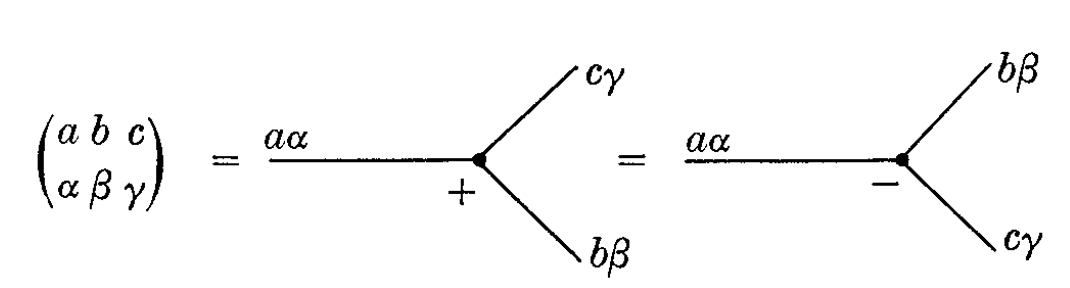
\includegraphics[scale=0.7]{j3_graph}
	\caption{The graphical Wigner $3j$-symbol \cite{angular_momentum}}
\end{figure}
The symmetry relation 
\begin{equation*}
\tj{a}{b}{c}{\al}{\be}{\gamma} = (-1)^{a+b+c}\tj{a}{c}{b}{\al}{\gamma}{\be}
\end{equation*}
implies that 
\begin{figure}[!htb]
	\centering
	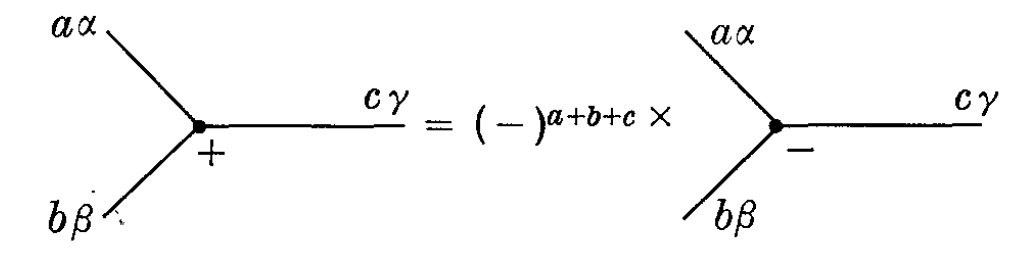
\includegraphics[scale=0.7]{j3_graph1}
	\caption{Symmetry relation for the graphical Wigner $3j$-symbol \cite{angular_momentum}}
\end{figure}
The sign $+/-$ at the node denotes the counterclockwise/clockwise orientation. The associated $3j$-symbol does not change under deformations of a diagram so long as such deformations do not alter the diagram's orientation. Next, sometimes we see various phase factors of the form $(-1)^{x+y+z+\dots}$. These are represented by arrows. In particular, 
\begin{figure}[!htb]
	\centering
	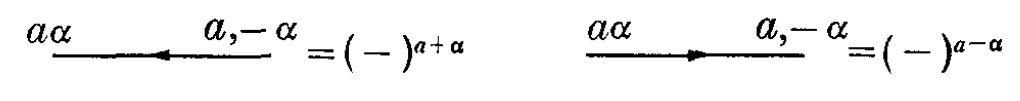
\includegraphics[scale=0.7]{j3_graph2}
	\caption{Phase factor as an arrow \cite{angular_momentum}}
\end{figure}
More complicated diagrams maybe constructed by putting these ingredients together. Two lines representing the same total angular momentum can be joined. Joining two lines implies that the $z$-components of the two angular momenta should be set equal and summed over. We will usually omit the $z$-components of angular momenta from diagrams. 

With these rules we should be able to write down any  Clebsch-Gordan coefficient in terms of $3j$-symbols. This is easy, so I won't do an example (for more details refer to \cite{angular_momentum}). What we'll focus on is the Wigner $6j$-symbol, which is given by Figure \ref{fig:6j}, where the sum is taken over all magnetic quantum numbers. 
\begin{figure}[!htb]
	\centering
	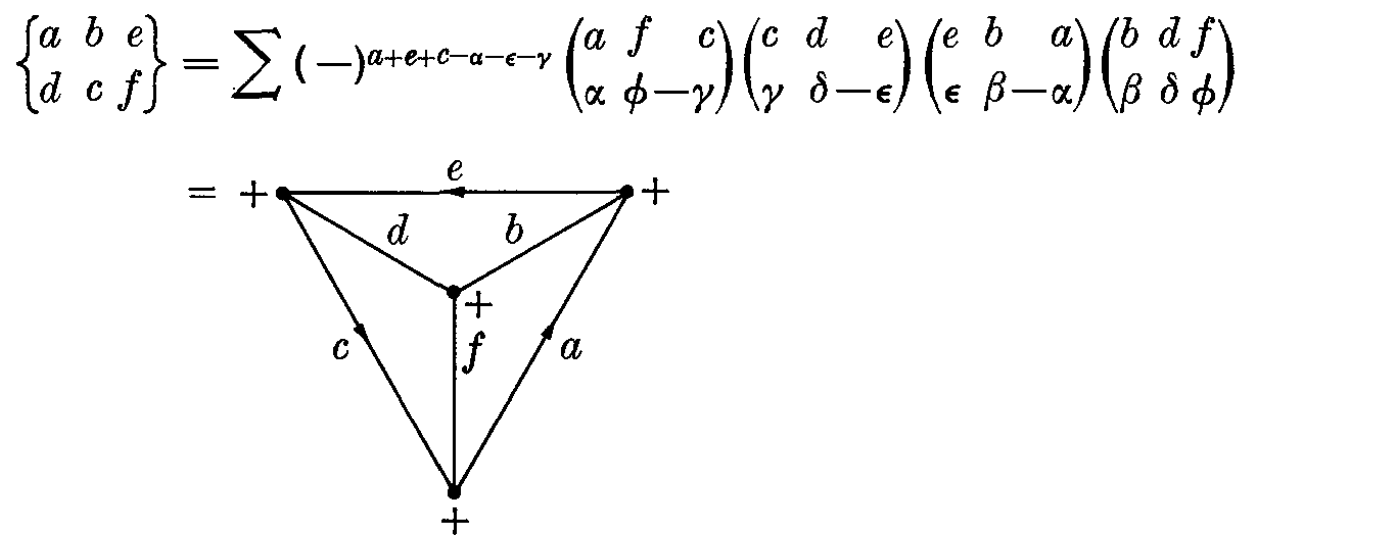
\includegraphics[scale=0.7]{j6_graph}
	\caption{The graphical Wigner $6j$-symbol \cite{angular_momentum}}
	\label{fig:6j}
\end{figure}


\subsection{Rules for transforming graphs}
Often in calculations, we start with an algebraic expression and translate it into a rather complicated graphical representation. To continue with the calculation, we often must transform the complicated graph into products of more elementary ones before this simpler graph is converted back into a simplified algebraic expression. Here are some rules to perform the transformations. 

First, we must know how to add/remove arrows or change their directions. There are \textbf{five} rules. The first four rules are best shown in diagrams (see Figures \ref{fig:arrow1}, \ref{fig:arrow2}, \ref{fig:arrow3}, \ref{fig:arrow4}). 
	\begin{figure}[!htb]
		\centering
		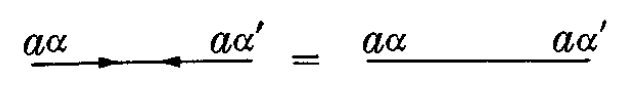
\includegraphics[scale=0.7]{arrow_1}
		\caption{Two opposite arrows ``cancel'' \cite{angular_momentum}}
		\label{fig:arrow1}
	\end{figure}	
	\begin{figure}[!htb]
		\centering
		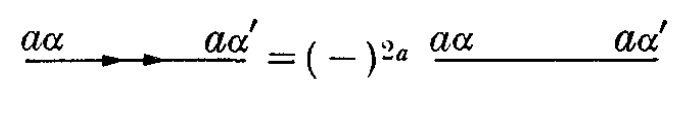
\includegraphics[scale=0.7]{arrow_2}
		\caption{Two arrows in the same direction  ``cancel'' and give a phase  \cite{angular_momentum}}
		\label{fig:arrow2}
	\end{figure}
	\begin{figure}[!htb]
		\centering
		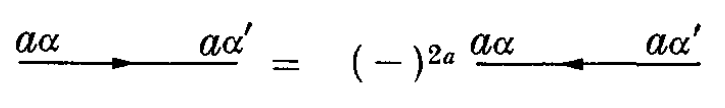
\includegraphics[scale=0.7]{arrow_3}
		\caption{Changing the direction of an arrow gives a phase \cite{angular_momentum}}
		\label{fig:arrow3}
	\end{figure}
	\begin{figure}[!htb]
		\centering
		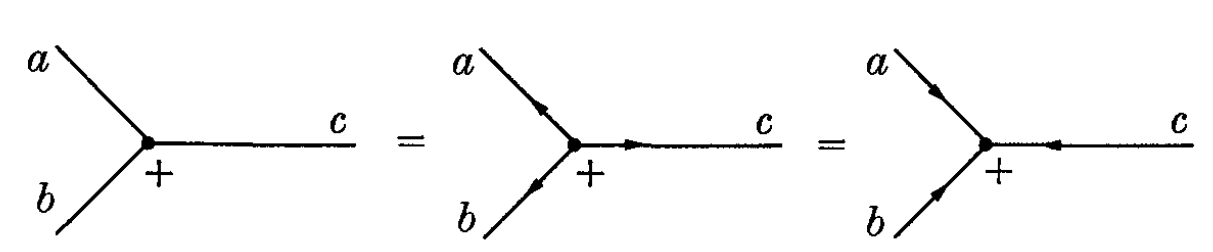
\includegraphics[scale=0.7]{arrow_4}
		\caption{3 arrows (\textit{all} away from or towards the node) might be added to the diagram  \cite{angular_momentum}}
		\label{fig:arrow4}
	\end{figure}
The fifth rule says that the direction of all arrows and the signs of all nodes may be changed simultaneously in a closed diagram without altering the value of the diagram. The proof for this rule is once again in \cite{angular_momentum}. 

Second, we must know how to ``factor'' a complicated diagram into smaller, more recognizable ones. This brings us to the the Three Theorems for Block Diagrams in \cite{angular_momentum}, but we'll just learn the rules by looking at some model diagrams. One important result is that if we denote a block $F$ with $n$ external lines by Figure \ref{fig:block0}, then Figure \ref{fig:block1} follows.
\begin{figure}[!htb]
	\centering
	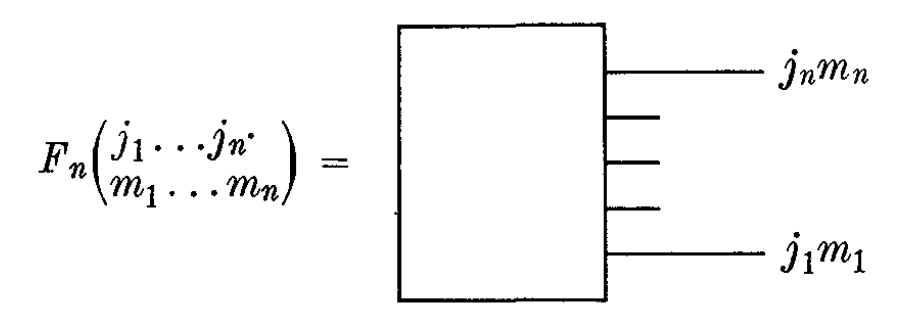
\includegraphics[scale=0.7]{block0}
	\caption{From \cite{angular_momentum}}
	\label{fig:block0}
\end{figure}
\begin{figure}[!htb]
	\centering
	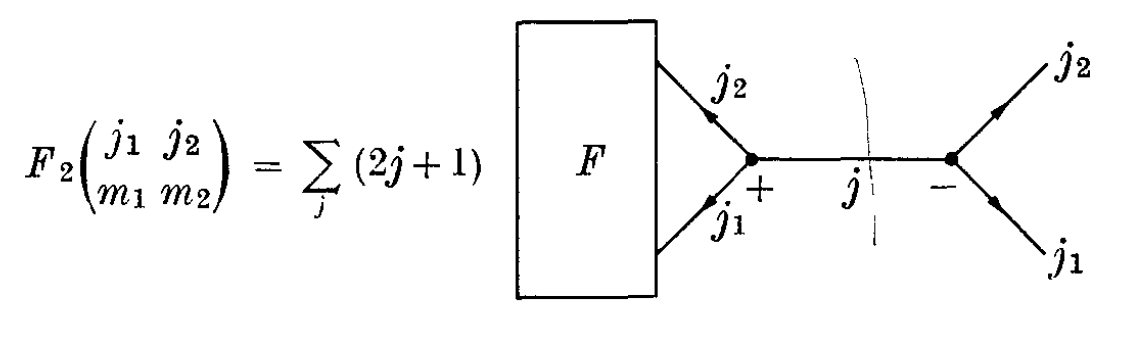
\includegraphics[scale=0.7]{block1}
	\caption{From \cite{angular_momentum}}
	\label{fig:block1}
\end{figure}



We focus on the cases where there are two (Figure \ref{fig:two}) and three (Figure \ref{fig:three}) connecting lines between two blocks. 
	\begin{figure}[!htb]
		\centering
		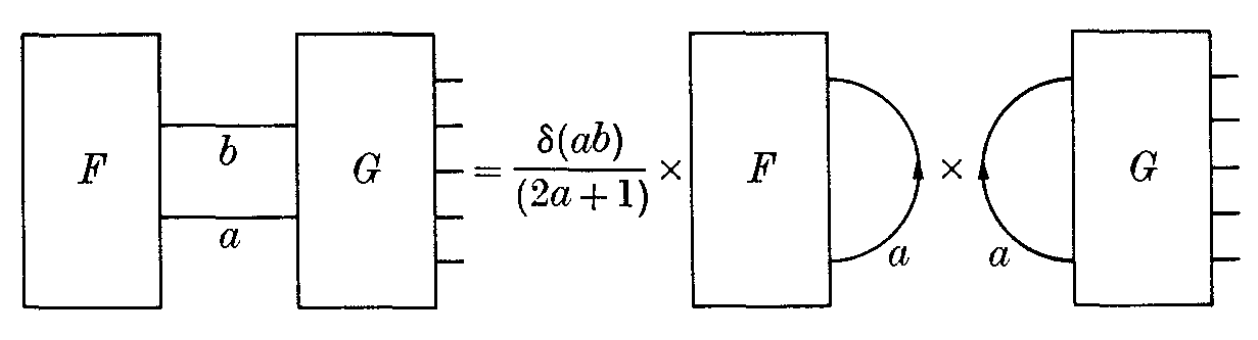
\includegraphics[scale=0.7]{blocks_two_lines}
		\caption{Two blocks with two connecting lines \cite{angular_momentum}}
		\label{fig:two}
	\end{figure}
	
	\begin{figure}[!htb]
		\centering
		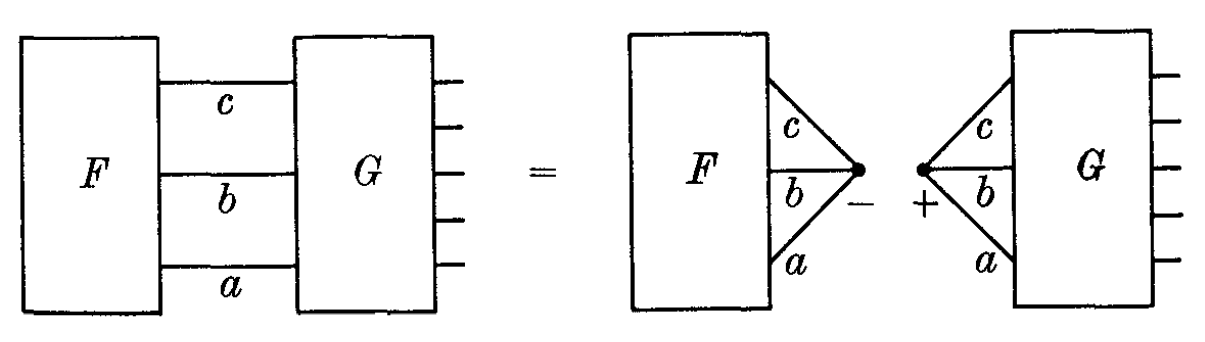
\includegraphics[scale=0.7]{blocks_three_lines}
		\caption{Two blocks with three connecting lines \cite{angular_momentum}}
		\label{fig:three}
	\end{figure}

In the case where we have a single block with 2 or 3 external lines, we can simply call this block $F$ and let the block $G$ be blank. By doing so, we can treat the external lines of block $F$ as connecting lines and apply the rules. For example, we can prove the relation
\begin{equation*}
\sum_{\delta\epsilon\phi}\tj{d}{e}{c}{-\delta}{\epsilon}{\gamma}\tj{e}{f}{a}{-\epsilon}{\phi}{\al}\tj{f}{d}{b}{-\phi}{\delta}{\beta}(-1)^{d+e+f-\delta-\epsilon-\phi} = \Gj{a}{b}{c}{d}{e}{f}\tj{a}{b}{c}{\al}{\be}{\gamma}
\end{equation*}
graphically in Figure \ref{fig:graph}.
\begin{figure}[!htb]
	\centering
	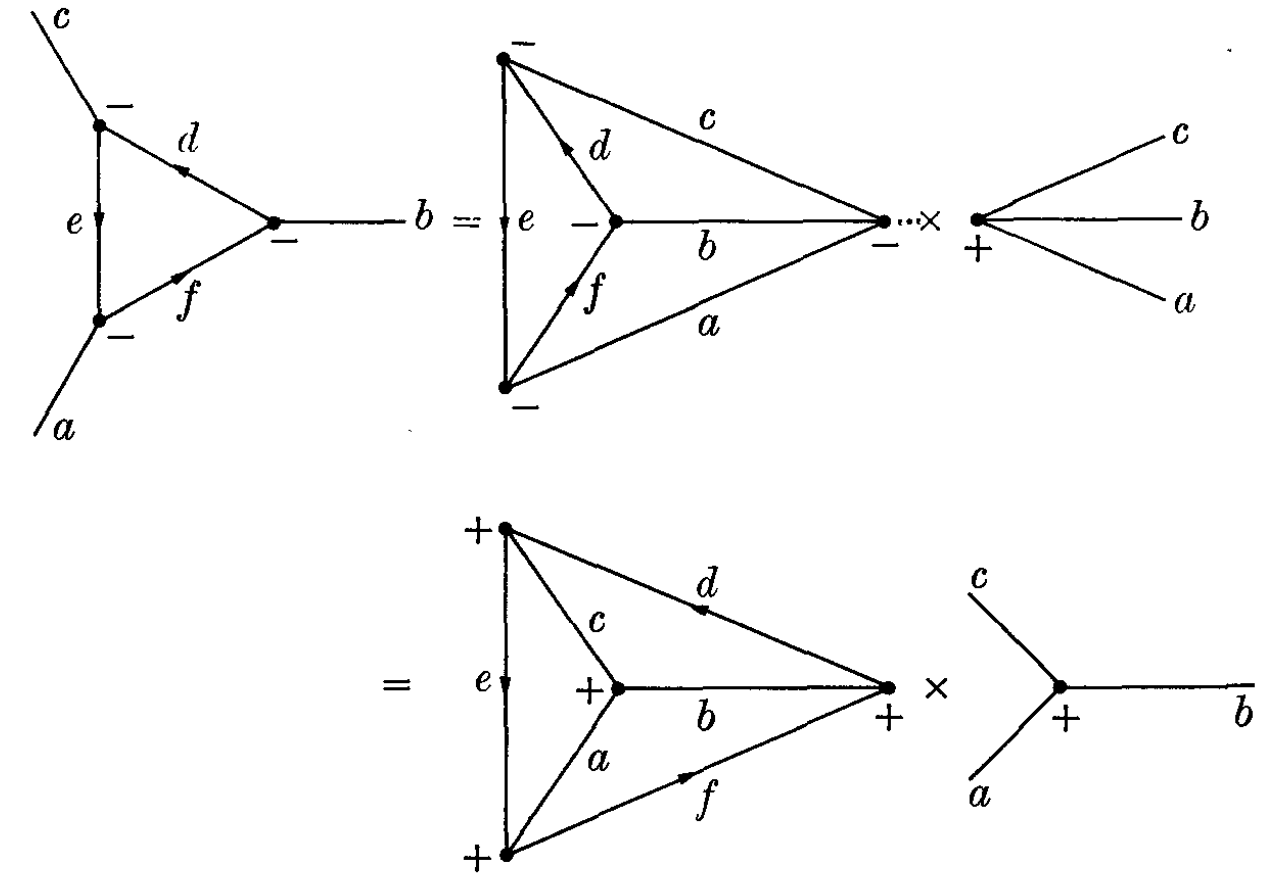
\includegraphics[scale=0.7]{blocks_ex}
	\caption{An example of using the block-diagram theorems \cite{angular_momentum}}
	\label{fig:graph}
\end{figure}

Another interesting example is calculating the block in Figure \ref{fig:block_ex}, which can be transformed into Figure \ref{fig:block_ex1}.
\begin{figure}[!htb]
	\centering
	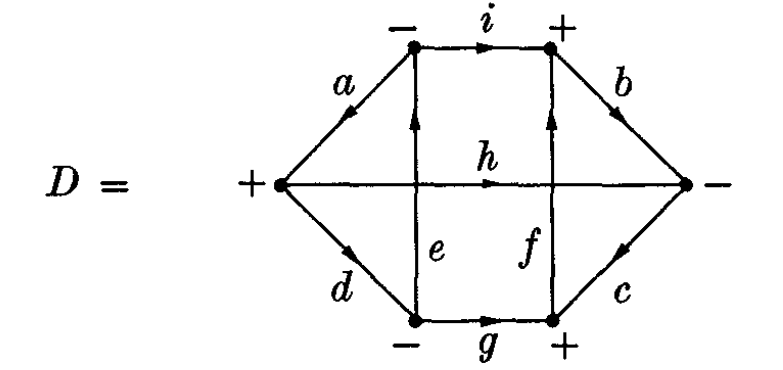
\includegraphics[scale=0.7]{blocks_ex1}
	\caption{From \cite{angular_momentum}}
	\label{fig:block_ex}
\end{figure}
\begin{figure}[!htb]
	\centering
	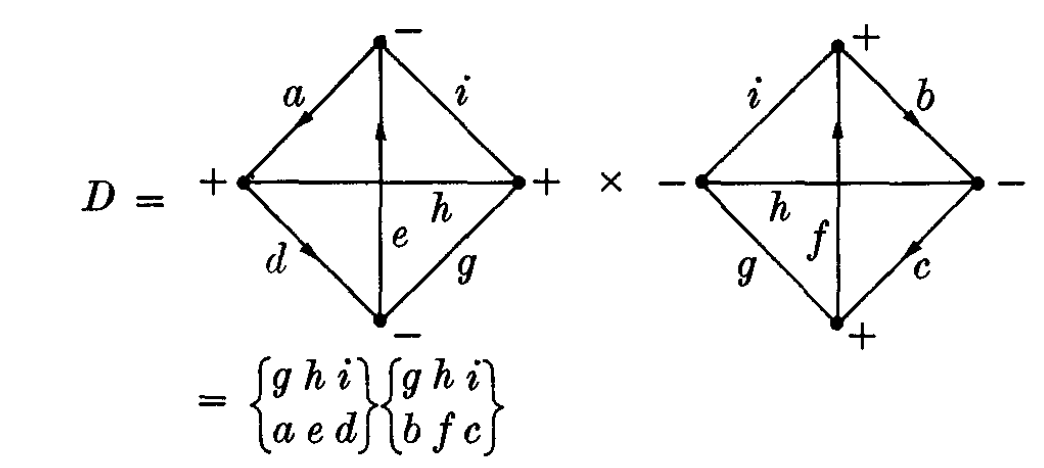
\includegraphics[scale=0.7]{blocks_ex2}
	\caption{From \cite{angular_momentum}}
	\label{fig:block_ex1}
\end{figure}
Here, we have used the sequence of transformation shown in Figure \ref{fig:justify}.
\begin{figure}[!htb]
	\centering
	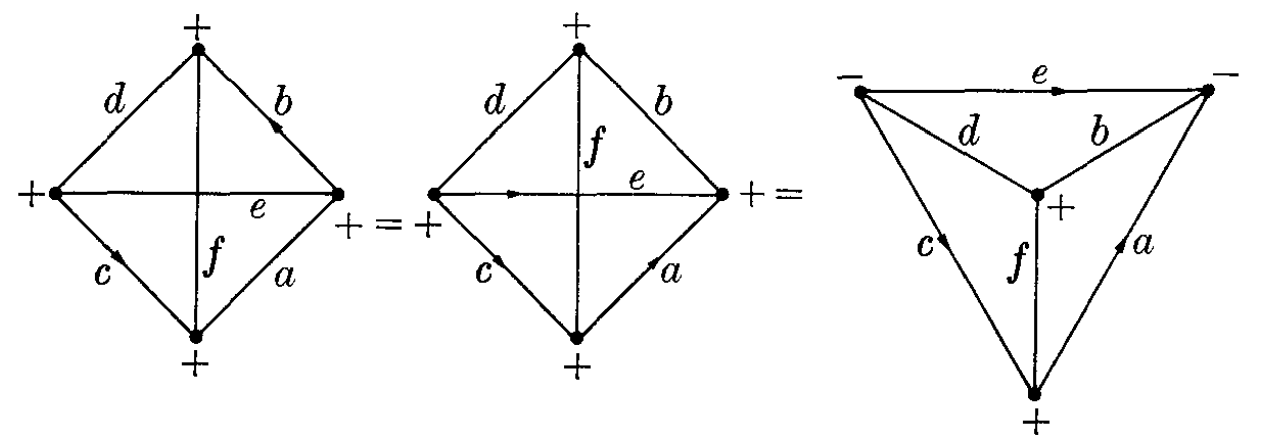
\includegraphics[scale=0.7]{transformation}
	\caption{From \cite{angular_momentum}}
	\label{fig:justify}
\end{figure}


\subsection{Calculating $X(F_e, F_e', F_i, F_f; p_0, p_0', p,p')$}\label{app:X}
We're now ready to calculate $X(F_e, F_e', F_i, F_f; p_0, p_0', p,p')$ in Section \ref{sec:beat_theory}. Recall that:
\begin{align*}
X(F_e,F'_e,F_i,F_f;p_0.p_o',p,p') &= \sum_{\substack{M_eM'_e\\ M_i M_f}}(-1)^{F_e - M_e + F'_e - M'_e + F_i - M_i + F_f - M_f} \tj{F_e}{1}{F_i}{-M_e}{p_0}{M_i}\\ 
&\quad \times 
\tj{F_i}{1}{F'_e}{-M_i}{p'_0}{M'_e}
\tj{F'_e}{1}{F_f}{-M'_e}{p}{M_f}
\tj{F_f}{1}{F_e}{-M_f}{p'}{M_e}.
\end{align*}
By using the graphical representations for the $3j$-symbol and an arrow, the term
\begin{align*}
(-1)^{F_e - M_e} \tj{F_e}{1}{F_i}{-M_e}{p_0}{M_i}
\end{align*}
is represented by the graph in Figure \ref{fig:X1}.
\begin{figure}[!htb]
	\centering
	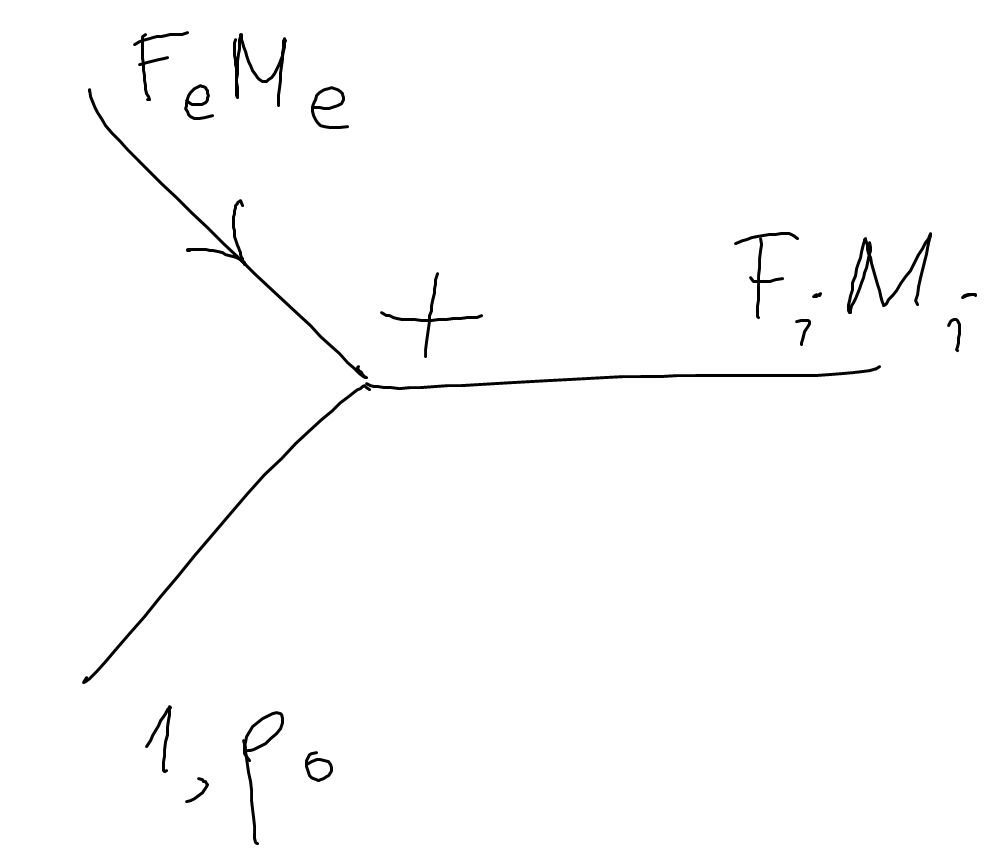
\includegraphics[scale=0.3]{draw_ang_1}
	\caption{}
	\label{fig:X1}
\end{figure}


Putting the four terms in $X$ together by joining lines we get to Figure \ref{fig:X2}. We can treat Figure \ref{fig:X2} as a two-block diagram with two connecting lines. Applying the block-diagram theorem, we obtain Figure \ref{fig:X3}. To simplify Figure \ref{fig:X3} further, we add three diverging arrows to the node $k-F_e-F_e'$ and invoke the ``external line rule'' used in Figure \ref{fig:graph}. This gives Figure \ref{fig:X4}.
\begin{figure}[!htb]
	\centering
	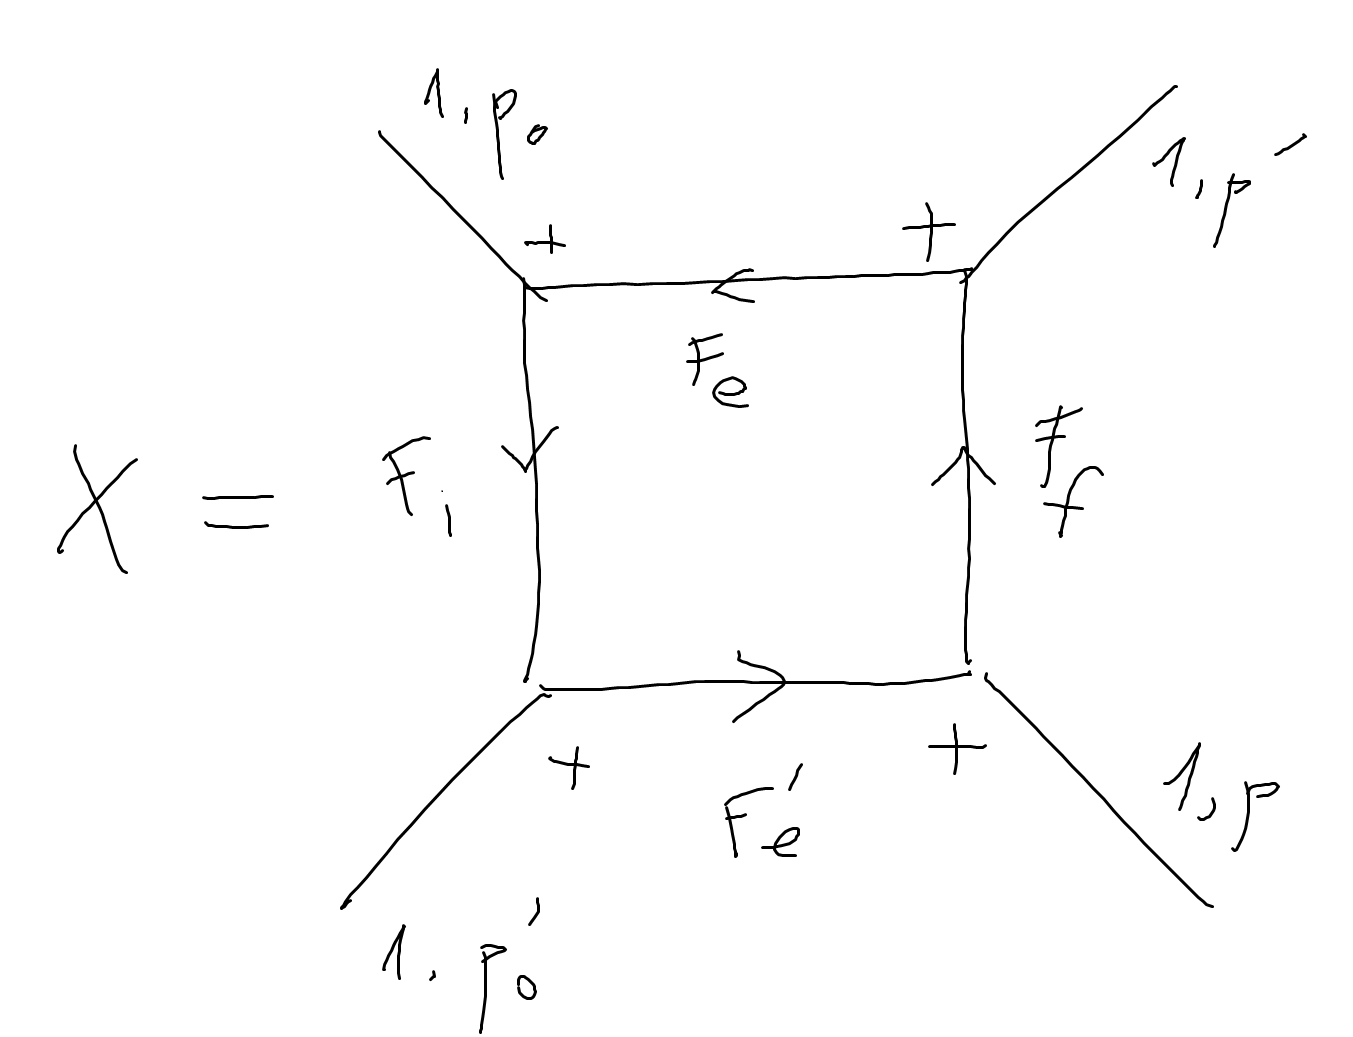
\includegraphics[scale=0.3]{draw_ang_2}
	\caption{}
	\label{fig:X2}
\end{figure}
\begin{figure}[!htb]
	\centering
	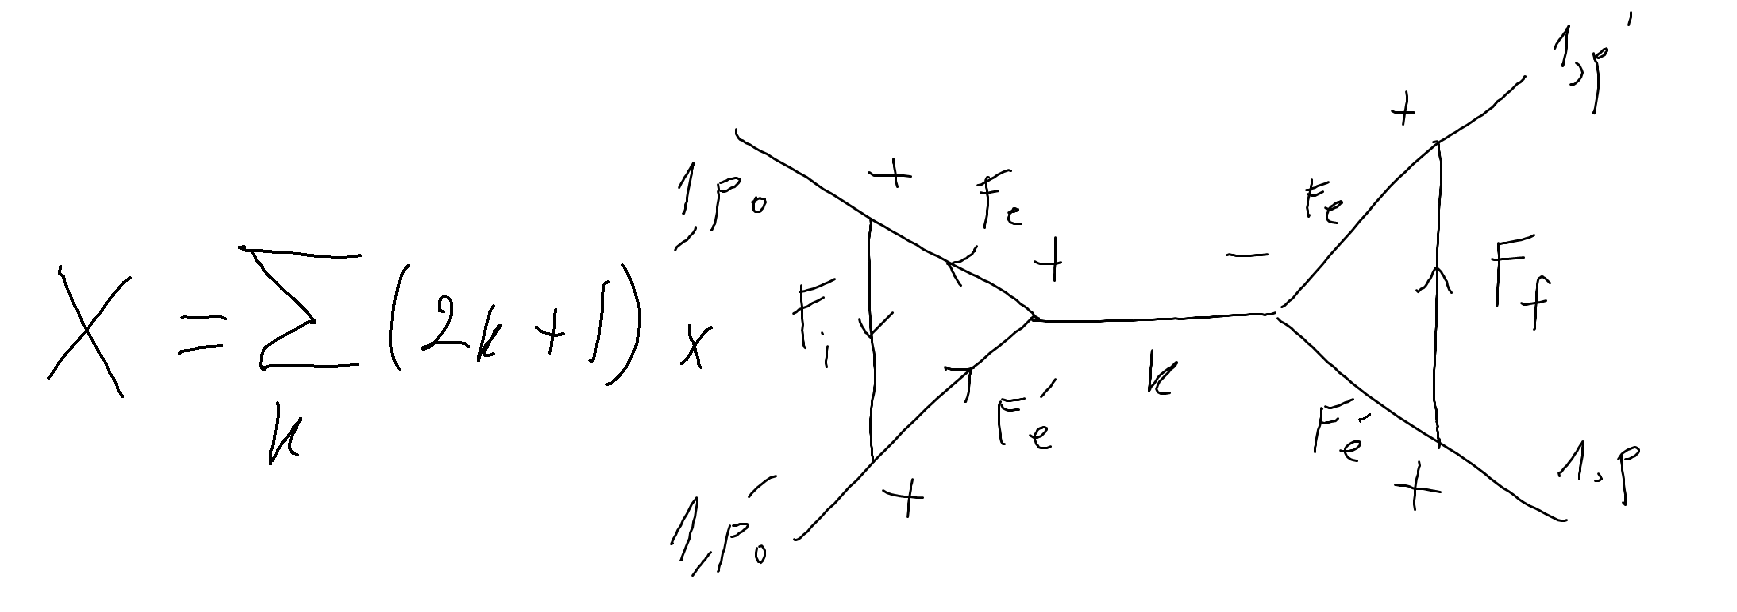
\includegraphics[scale=0.4]{draw_ang_3}
	\caption{}
	\label{fig:X3}
\end{figure}
\begin{figure}[!htb]
	\centering
	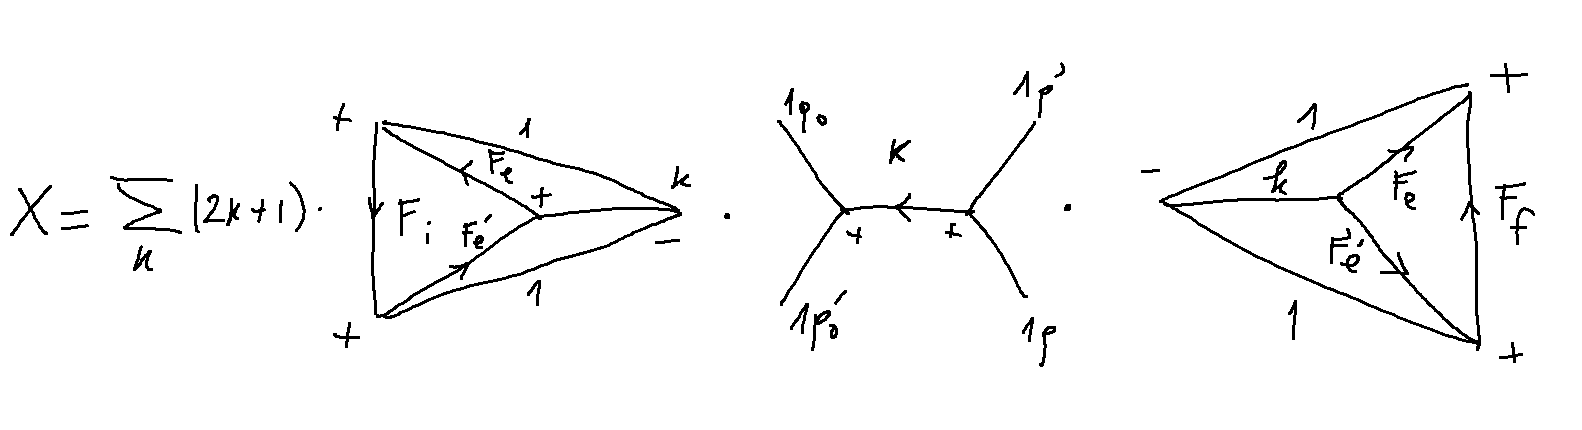
\includegraphics[scale=0.6]{draw_ang_4}
	\caption{}
	\label{fig:X4}
\end{figure}  
Next, to the left-most term, add diverging arrows to the $F_i-F_e-1$ node and converging arrows to the $1-F'_e-F_i$ node. This has no effect on the $F_i$ line. However, the arrows on the $F_e$ and $F_e'$ lines get canceled, and we gain new arrows on the ``outer'' $1$-lines. Repeat this process for the right-most term so that its ``inner arrows''  also get canceled. Notice further that switching arrow directions on the $1$-line doesn't do anything to the graph because the phase $(-1)^{2\times 1} = 1$. Using this fact, we can also change the orientations of the nodes with the $-$ sign so that they become $+$. After some extra careful changing of signs and arrow directions, we will find the ``triangular terms'' in the correct form for the $6j$-symbol. We also recognize that the term in the middle is just the product of two $3j$-symbols. So, in the end, we write
\begin{align*}
X(F_e,F'_e,F_i,F_f;p_0.p_o',p,p') &= \sum_{kq} (2k+1) (-1)^{q + 2F_f - F_e - F_e'}\tj{1}{1}{k}{p_0}{p_0'}{q}\tj{1}{1}{k}{p}{p'}{-q}  \\
&\quad\times \Gj{F_i}{F_e}{1}{k}{1}{F_e'} \Gj{1}{k}{1}{F_e}{F_f}{F_e'}.
\end{align*}

\subsection{Calculating $Y(F_e, F_e';k)$ and $Z(F_e, F_e';k)$} \label{app:YZ}
Recall their formulas from Section \ref{sec:beat_theory}:
\begin{equation*}
Y(F_e, F_e';k) = \sum_{F_i}(2F_i + 1)(-1)^{2J_e + k + F_e + F_e' + I + J_i + F_i}
\Gj{F_e}{F_i}{1}{J_i}{J_e}{I}
\Gj{F_e'}{F_i}{1}{1}{k}{F_e}
\Gj{I}{F_i}{J_i}{1}{J_e}{F_e'}.
\end{equation*}
and
\begin{equation*}
Z(F_e, F_e';k) = \sum_{F_f}(2F_f + 1)(-1)^{2J_e + k + F_e + F_e' + I + J_f + F_f}
\Gj{F'_e}{F_f}{1}{J_f}{J_e}{I}
\Gj{F_e}{F_f}{1}{1}{k}{F_e'}
\Gj{I}{F_f}{J_f}{1}{J_e}{F_e}.
\end{equation*}
We will perform these calculations based on Example 7 of Chapter VII: Graphical Methods in Angular Momentum in \cite{angular_momentum}. It suffices to just do the $Y$ calculation. The result for $Z$ can be obtained by a simple change of variables. To start, we look at Example 7, which says that
\begin{equation*}
\sum_{x}(2x+1)(-1)^{a+b+c+d+e+f+g+h+i+x}
\Gj{e}{f}{x}{b}{a}{i} 
\Gj{a}{b}{x}{c}{d}{h} 
\Gj{d}{c}{x}{f}{e}{g} 
=
\Gj{g}{h}{i}{a}{e}{d} 
\Gj{g}{h}{i}{b}{f}{c}.
\end{equation*}
We want to do some permutations to the $6j$-symbols in $Y$ so that it matches the expression above. We first recognize that $F_i$ plays the role of $x$. 
\begin{align*}
Y(F_e, F_e';k) 
&= 
\sum_{F_i}(2F_i + 1)(-1)^{2J_e + k + F_e + F_e' + I + J_i + F_i}
\Gj{F_e}{1}{F_i}{J_i}{I}{J_e}
\Gj{I}{J_i}{F_i}{1}{F_e'}{J_e}
\Gj{F_e'}{1}{F_i}{1}{F_e}{k}\\
&= 
\Gj{k}{J_e}{J_e}{I}{F_e}{F_e'} 
\Gj{k}{J_e}{J_e}{J_i}{1}{1}.
\end{align*}
For $Z$, we observe that $F_e$ and $F_e'$ are exchanged, $J_i$ is replaced by $J_f$, and that $F_f$ plays the role of $x$. But since the $6j$-symbol is invariant under permutations of columns, the $F_e - F_e'$ exchange in fact has no effect. So,
\begin{align*}
Z(F_e, F_e';k) 
= 
\Gj{k}{J_e}{J_e}{I}{F_e'}{F_e} 
\Gj{k}{J_e}{J_e}{J_f}{1}{1}
=
\Gj{k}{J_e}{J_e}{I}{F_e}{F_e'} 
\Gj{k}{J_e}{J_e}{J_f}{1}{1}.
\end{align*}

To see how one might do this graphically, we observe that 
\begin{equation*}
\sum_{x}(2x+1)(-1)^{a+b+c+d+e+f+g+h+i+x}
\Gj{e}{f}{x}{b}{a}{i} 
\Gj{a}{b}{x}{c}{d}{h} 
\Gj{d}{c}{x}{f}{e}{g} 
\end{equation*}
can be written as Figure \ref{fig:transf} \cite{angular_momentum}.
\begin{figure}[!htb]
	\centering
	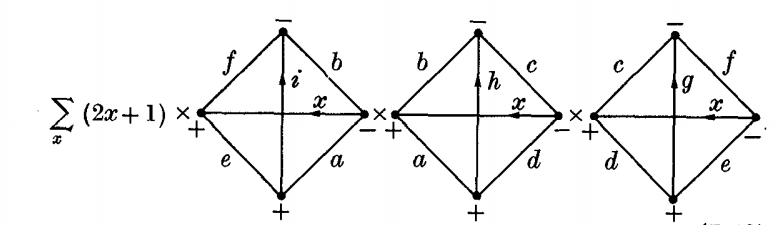
\includegraphics[scale=0.7]{transformation_1}
	\caption{}
	\label{fig:transf}
\end{figure}
To obtain this result, we just write out the $6j$-symbols as the ``triangular'' graphs as before. Next, the phase factors will change some of the orientations, which convert from $+$ nodes to $-$ and move the ``inner node'' outside of the triangle, turning it into a square. That's the idea. \textcolor{blue}{I believe that this is good enough of an instruction. The rest is left to the reader.} Next, the graph in Figure \ref{fig:transf} \cite{angular_momentum} can be ``contracted'' into the graph in Figure \ref{fig:transf1}. To go from Figure \ref{fig:transf} to Figure \ref{fig:transf1}, we use the Block-Diagram Theorems and join the 3 graphs into the form in Figure \ref{fig:transf2} \cite{angular_momentum}, which can then be separated on the lines $(ghi)$ to give Figure \ref{fig:transf1}. After some change of orientations at the nodes of Figure \ref{fig:transf1} we get the desired result: 
\begin{align*}
\Gj{g}{h}{i}{a}{e}{d} 
\Gj{g}{h}{i}{b}{f}{c}.
\end{align*}
\begin{figure}[!htb]
	\centering
	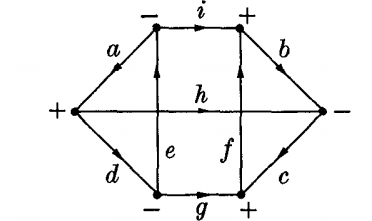
\includegraphics[scale=0.7]{transformation_3}
	\caption{}
	\label{fig:transf2}
\end{figure}
\begin{figure}[!htb]
	\centering
	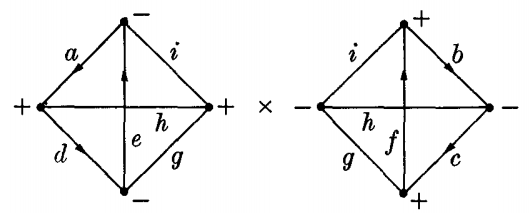
\includegraphics[scale=0.7]{transformation_2}
	\caption{}
	\label{fig:transf1}
\end{figure}










\section{Spherical Basis and the Wigner $\mathcal{D}$-matrix}\label{app:Spherical}

A spherical basis is the basis used to express spherical tensors. Spherical bases are ubiquitous in angular-momentum problems in quantum mechanics. While spherical polar coordinates are one orthogonal coordinate system for expressing vectors and tensors using polar and azimuthal angles and radial distance, the spherical basis are constructed from the standard basis and use complex numbers. In three dimensions, a vector $\mathbf{A}$ in the standard basis can be written as
\begin{equation*}
\mathbf{A} = {A}_x \mathbf{e}_x + {A}_y \mathbf{e}_y + {A}_z \mathbf{e}_z.
\end{equation*}
where the coordinates $A_i$ can be complex. In the spherical basis denoted $\mathbf{e}_+, \mathbf{e}_-, \mathbf{e}_0$, 
\begin{equation*}
\mathbf{A} = {A}_+ \mathbf{e}_+ + 
{A}_- \mathbf{e}_- + {A}_0 \mathbf{e}_0
\end{equation*}
where
\begin{equation*}
\mathbf{e}_\pm = \mp \f{1}{\sqrt{2}} (\mathbf{e}_x \pm i\mathbf{e}_y)
\end{equation*}
and
\begin{equation*}
\mathbf{e}_0 = \mathbf{e}_z.
\end{equation*}
This change of basis can be captured by 
\begin{equation*}
\begin{pmatrix}
\mathbf{e}_+ \\ \mathbf{e}_- \\ \mathbf{e}_0
\end{pmatrix}
=
\mathbf{U}
\begin{pmatrix}
\mathbf{e}_x \\ \mathbf{e}_y \\ \mathbf{e}_z
\end{pmatrix}
= 
\begin{pmatrix}
-1/\sqrt{2} & -i/\sqrt{2} & 0\\
+1/\sqrt{2} & -i/\sqrt{2} & 0\\
0 & 0 & 1
\end{pmatrix}
\begin{pmatrix}
\mathbf{e}_x \\ \mathbf{e}_y \\ \mathbf{e}_z
\end{pmatrix}.
\end{equation*}
The corresponding change of coordinates is 
\begin{equation*}
\begin{pmatrix}
{A}_+ \\ {A}_- \\ {A}_0
\end{pmatrix}
=
\mathbf{U}^*
\begin{pmatrix}
{A}_x \\ {A}_y \\ {A}_z
\end{pmatrix}.
\end{equation*}
We notice that $U$ is unitary, i.e., $U^\dagger = U^{-1}$.  


A general spherical tensor transforms under a rotation the same way spherical harmonics transform. It turns out that if $T^k_q$ is a spherical tensor, then 
\begin{equation}\label{eq:def}
\mathcal{D}(\mathbf{R})T^k_q \mathcal{D}^\dagger(\mathbf{R}) = \sum_{q' = -k}^k T^k_{q'} \mathcal{D}^k_{qq'}(\mathbf{R}) 
\end{equation}
where $\mathbf{R}$ is a 3-dimensional rotation operator and $\mathcal{D}$ is the Wigner $\mathcal{D}$-matrix associated with the rotation matrix $\mathbf{D}$. With corresponding Euler angles $\al,\be,\gamma$, $\mathbf{R}$ can be written as 
\begin{equation*}
\mathbf{R}(\al,\be,\gamma) = e^{-i\al \sigma_z}e^{-i\beta \sigma_y} e^{-i\gamma \sigma_z}.
\end{equation*}
The Euler angles are characterized by the keywords: $z-y-z$ convention, right-handed frame, right-hand screw rule, active interpretation. Here $\sigma_i$ are the Pauli matrices, which are also generators of the Lie algebra of SO(3). Let's unpack the right-hand side of Eq. \ref{eq:def}. $\mathcal{D}$ is a unitary square matrix of dimension $2k+1$ in this spherical basis with elements $\mathcal{D}^k_{qq'}(\mathbf{R})$, defined by 
\begin{equation*}
\mathcal{D}^k_{qq'}(\al,\be,\gamma) \equiv \bra{kq} \mathbf{R}(\al,\be,\gamma) \ket{kq'} = e^{-iq\al} \bra{kq} e^{-i\be \sigma_y} \ket{kq'} e^{-iq'\gamma} = e^{-iq\al} \mathcal{D}^j_{qq'}(0,\be,0) e^{-iq'\gamma}.
\end{equation*}
Here $\mathcal{D}^j_{qq'}(0,\be,0)$ is referred to as the \textbf{Wigner's (small) $d$-matrix}:
\begin{equation*}
d^k_{qq'}(\be) = \mathcal{D}^j_{qq'}(0,\be,0).
\end{equation*}
Elements of $d^k_{qq'}(\be)$ can be readily found. In the case where $k = 2$ and $q=q' =0$, we have
\begin{equation*}
d^2_{00}(\be) = \f{1}{2}(3\cos^2\be - 1) = P_2(\cos\beta).
\end{equation*}
\textcolor{blue}{Note to the reader: Does this look familiar?} It turns out that 
\begin{equation*}
\mathcal{D}^k_{00}(\varphi,\theta,\phi) = P_k(\cos\theta)
\end{equation*}
where $P_k(x)$ are Legendre polynomials. In general, 
\begin{equation*}
\mathcal{D}^l_{m0}(\al,\be,\gamma) = \sqrt{\f{(l-m)!}{(l+m)!}} P^m_l(\cos\beta) e^{-im\al},
\end{equation*}
which implies that
\begin{equation*}
d^l_{m0}(\be) = \sqrt{\f{(l-m)!}{(l+m)!}} P^m_l(\cos\beta).
\end{equation*}
Here, $P^m_l(x)$ are the associated Legendre polynomials. 








\end{appendices}







\bibliographystyle{unsrt}
\bibliography{quantum_beats}
\end{document}